% Options for packages loaded elsewhere
\PassOptionsToPackage{unicode}{hyperref}
\PassOptionsToPackage{hyphens}{url}
%
\documentclass[
]{article}
\usepackage{amsmath,amssymb}
\usepackage{iftex}
\ifPDFTeX
  \usepackage[T1]{fontenc}
  \usepackage[utf8]{inputenc}
  \usepackage{textcomp} % provide euro and other symbols
\else % if luatex or xetex
  \usepackage{unicode-math} % this also loads fontspec
  \defaultfontfeatures{Scale=MatchLowercase}
  \defaultfontfeatures[\rmfamily]{Ligatures=TeX,Scale=1}
\fi
\usepackage{lmodern}
\ifPDFTeX\else
  % xetex/luatex font selection
\fi
% Use upquote if available, for straight quotes in verbatim environments
\IfFileExists{upquote.sty}{\usepackage{upquote}}{}
\IfFileExists{microtype.sty}{% use microtype if available
  \usepackage[]{microtype}
  \UseMicrotypeSet[protrusion]{basicmath} % disable protrusion for tt fonts
}{}
\makeatletter
\@ifundefined{KOMAClassName}{% if non-KOMA class
  \IfFileExists{parskip.sty}{%
    \usepackage{parskip}
  }{% else
    \setlength{\parindent}{0pt}
    \setlength{\parskip}{6pt plus 2pt minus 1pt}}
}{% if KOMA class
  \KOMAoptions{parskip=half}}
\makeatother
\usepackage{xcolor}
\usepackage[margin=1in]{geometry}
\usepackage{color}
\usepackage{fancyvrb}
\newcommand{\VerbBar}{|}
\newcommand{\VERB}{\Verb[commandchars=\\\{\}]}
\DefineVerbatimEnvironment{Highlighting}{Verbatim}{commandchars=\\\{\}}
% Add ',fontsize=\small' for more characters per line
\usepackage{framed}
\definecolor{shadecolor}{RGB}{248,248,248}
\newenvironment{Shaded}{\begin{snugshade}}{\end{snugshade}}
\newcommand{\AlertTok}[1]{\textcolor[rgb]{0.94,0.16,0.16}{#1}}
\newcommand{\AnnotationTok}[1]{\textcolor[rgb]{0.56,0.35,0.01}{\textbf{\textit{#1}}}}
\newcommand{\AttributeTok}[1]{\textcolor[rgb]{0.13,0.29,0.53}{#1}}
\newcommand{\BaseNTok}[1]{\textcolor[rgb]{0.00,0.00,0.81}{#1}}
\newcommand{\BuiltInTok}[1]{#1}
\newcommand{\CharTok}[1]{\textcolor[rgb]{0.31,0.60,0.02}{#1}}
\newcommand{\CommentTok}[1]{\textcolor[rgb]{0.56,0.35,0.01}{\textit{#1}}}
\newcommand{\CommentVarTok}[1]{\textcolor[rgb]{0.56,0.35,0.01}{\textbf{\textit{#1}}}}
\newcommand{\ConstantTok}[1]{\textcolor[rgb]{0.56,0.35,0.01}{#1}}
\newcommand{\ControlFlowTok}[1]{\textcolor[rgb]{0.13,0.29,0.53}{\textbf{#1}}}
\newcommand{\DataTypeTok}[1]{\textcolor[rgb]{0.13,0.29,0.53}{#1}}
\newcommand{\DecValTok}[1]{\textcolor[rgb]{0.00,0.00,0.81}{#1}}
\newcommand{\DocumentationTok}[1]{\textcolor[rgb]{0.56,0.35,0.01}{\textbf{\textit{#1}}}}
\newcommand{\ErrorTok}[1]{\textcolor[rgb]{0.64,0.00,0.00}{\textbf{#1}}}
\newcommand{\ExtensionTok}[1]{#1}
\newcommand{\FloatTok}[1]{\textcolor[rgb]{0.00,0.00,0.81}{#1}}
\newcommand{\FunctionTok}[1]{\textcolor[rgb]{0.13,0.29,0.53}{\textbf{#1}}}
\newcommand{\ImportTok}[1]{#1}
\newcommand{\InformationTok}[1]{\textcolor[rgb]{0.56,0.35,0.01}{\textbf{\textit{#1}}}}
\newcommand{\KeywordTok}[1]{\textcolor[rgb]{0.13,0.29,0.53}{\textbf{#1}}}
\newcommand{\NormalTok}[1]{#1}
\newcommand{\OperatorTok}[1]{\textcolor[rgb]{0.81,0.36,0.00}{\textbf{#1}}}
\newcommand{\OtherTok}[1]{\textcolor[rgb]{0.56,0.35,0.01}{#1}}
\newcommand{\PreprocessorTok}[1]{\textcolor[rgb]{0.56,0.35,0.01}{\textit{#1}}}
\newcommand{\RegionMarkerTok}[1]{#1}
\newcommand{\SpecialCharTok}[1]{\textcolor[rgb]{0.81,0.36,0.00}{\textbf{#1}}}
\newcommand{\SpecialStringTok}[1]{\textcolor[rgb]{0.31,0.60,0.02}{#1}}
\newcommand{\StringTok}[1]{\textcolor[rgb]{0.31,0.60,0.02}{#1}}
\newcommand{\VariableTok}[1]{\textcolor[rgb]{0.00,0.00,0.00}{#1}}
\newcommand{\VerbatimStringTok}[1]{\textcolor[rgb]{0.31,0.60,0.02}{#1}}
\newcommand{\WarningTok}[1]{\textcolor[rgb]{0.56,0.35,0.01}{\textbf{\textit{#1}}}}
\usepackage{graphicx}
\makeatletter
\def\maxwidth{\ifdim\Gin@nat@width>\linewidth\linewidth\else\Gin@nat@width\fi}
\def\maxheight{\ifdim\Gin@nat@height>\textheight\textheight\else\Gin@nat@height\fi}
\makeatother
% Scale images if necessary, so that they will not overflow the page
% margins by default, and it is still possible to overwrite the defaults
% using explicit options in \includegraphics[width, height, ...]{}
\setkeys{Gin}{width=\maxwidth,height=\maxheight,keepaspectratio}
% Set default figure placement to htbp
\makeatletter
\def\fps@figure{htbp}
\makeatother
\setlength{\emergencystretch}{3em} % prevent overfull lines
\providecommand{\tightlist}{%
  \setlength{\itemsep}{0pt}\setlength{\parskip}{0pt}}
\setcounter{secnumdepth}{-\maxdimen} % remove section numbering
\newlength{\cslhangindent}
\setlength{\cslhangindent}{1.5em}
\newlength{\csllabelwidth}
\setlength{\csllabelwidth}{3em}
\newlength{\cslentryspacingunit} % times entry-spacing
\setlength{\cslentryspacingunit}{\parskip}
\newenvironment{CSLReferences}[2] % #1 hanging-ident, #2 entry spacing
 {% don't indent paragraphs
  \setlength{\parindent}{0pt}
  % turn on hanging indent if param 1 is 1
  \ifodd #1
  \let\oldpar\par
  \def\par{\hangindent=\cslhangindent\oldpar}
  \fi
  % set entry spacing
  \setlength{\parskip}{#2\cslentryspacingunit}
 }%
 {}
\usepackage{calc}
\newcommand{\CSLBlock}[1]{#1\hfill\break}
\newcommand{\CSLLeftMargin}[1]{\parbox[t]{\csllabelwidth}{#1}}
\newcommand{\CSLRightInline}[1]{\parbox[t]{\linewidth - \csllabelwidth}{#1}\break}
\newcommand{\CSLIndent}[1]{\hspace{\cslhangindent}#1}
\ifLuaTeX
  \usepackage{selnolig}  % disable illegal ligatures
\fi
\IfFileExists{bookmark.sty}{\usepackage{bookmark}}{\usepackage{hyperref}}
\IfFileExists{xurl.sty}{\usepackage{xurl}}{} % add URL line breaks if available
\urlstyle{same}
\hypersetup{
  pdftitle={Rice farming with crop rotation for smallholder farmers in Indonesia},
  pdfauthor={Noviria Syifaun Nafsi, Sineenad Kongtonkun, Inkyin May, Vani Lian},
  hidelinks,
  pdfcreator={LaTeX via pandoc}}

\title{Rice farming with crop rotation for smallholder farmers in
Indonesia}
\author{Noviria Syifaun Nafsi, Sineenad Kongtonkun, Inkyin May, Vani
Lian}
\date{2023-07-13}

\begin{document}
\maketitle

\hypertarget{introduction}{%
\subsection{Introduction}\label{introduction}}

\hypertarget{overview}{%
\subsubsection{Overview}\label{overview}}

Indonesia is the largest country in Southeast Asia. Rice is the primary
staple food crop with a steady increase in annual production, making
Indonesia the third largest rice producer in the world. 93\% of
Indonesia's total number of farmers are small family farms. Rice is the
main crop grown and staple food in Southeast Asia.(Yoshida (1981)) Crop
rotation is the practice of planting different crops sequentially on the
same plot of land to improve soil health, optimize nutrients in the
soil, and combat pest and weed pressure.(Crystal and Whittlesey (2004))
Soybean is a species of legume native to East Asia, widely grown for its
edible bean which has numerous uses.(Wright et al. (2005)) Chili is a
plant of tropical and subtropical regions for their fleshy fruits.(MOALF
(2016))

\hypertarget{motivation}{%
\subsubsection{Motivation}\label{motivation}}

\begin{enumerate}
\def\labelenumi{\arabic{enumi}.}
\tightlist
\item
  Rice is the primary staple food crop with a steady increase in annual
  production, making Indonesia the third largest rice producer in the
  world.
\item
  Crop rotation can increase crop yields and income than monoculture of
  rice and it can help disrupt the lifecycle of crop pests and reducing
  chemical use.
\item
  Soybean can increase soil fertility and give extra income to farmers.
\item
  Chili cultivation can improve farmers' income because of good market
  price.
\end{enumerate}

\hypertarget{overview-of-the-project}{%
\subsubsection{Overview of the project}\label{overview-of-the-project}}

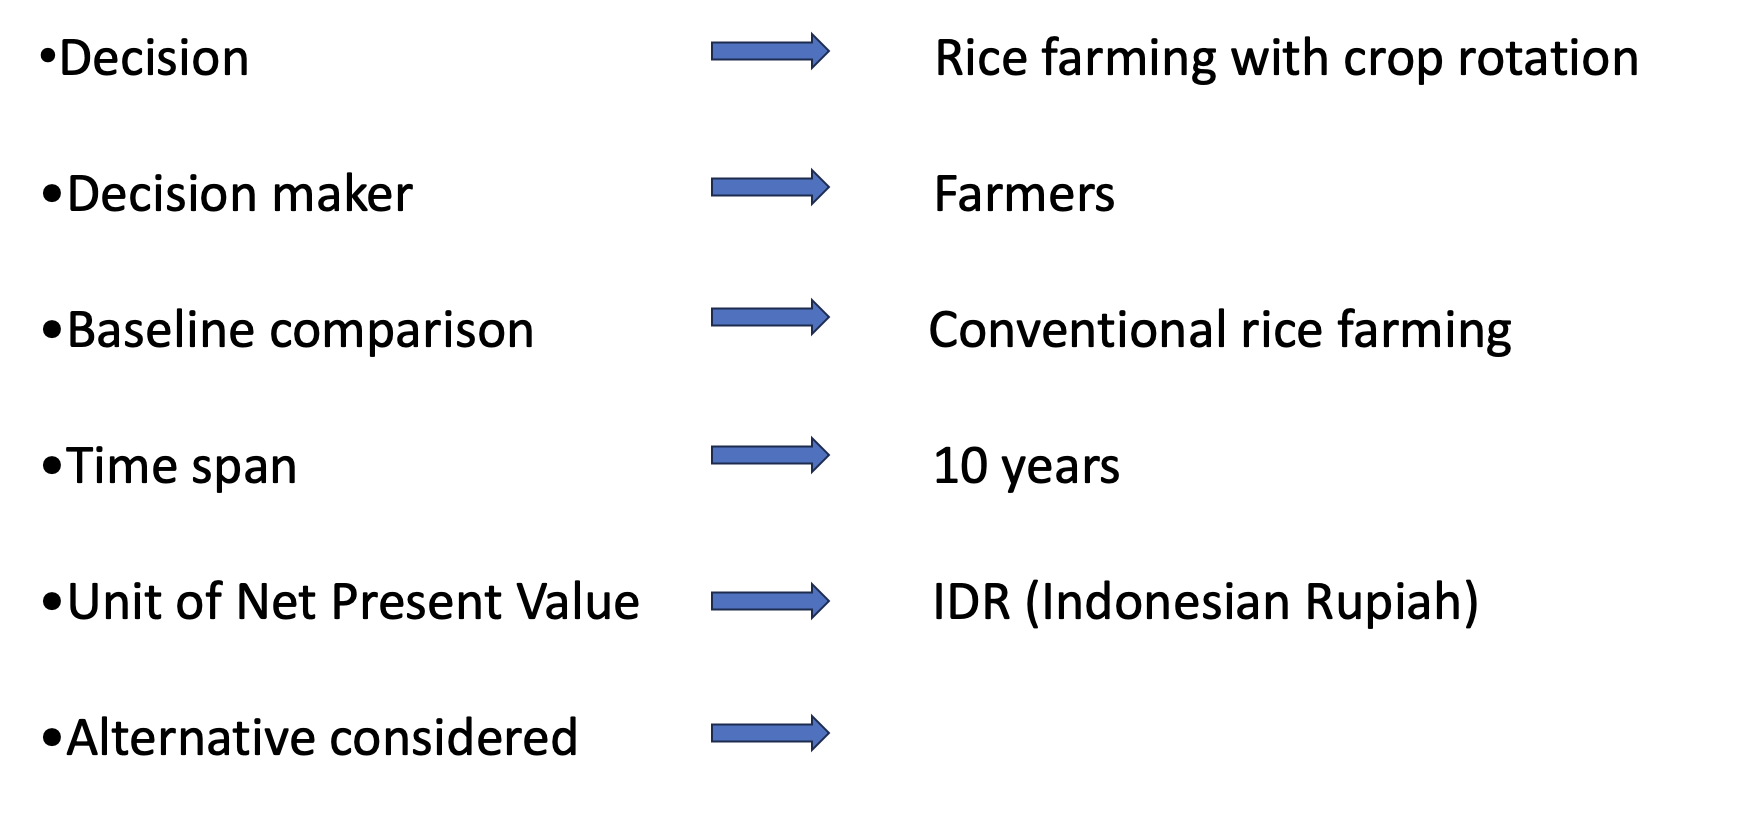
\includegraphics{Photo rice farm with crop rotation/overview of the project.png}

\hypertarget{conceptual-model}{%
\subsubsection{Conceptual model}\label{conceptual-model}}

This project will analyse the decision of crop rotation (soybean and
chili) with rice farming. Total cost is calculated for each crop, which
consists of labor, seeds, pesticides, fertilizer, machinery and rent
land. The revenues is calculated for each crop production by multiplying
the yield of each crop by the selling price of each crop per ha. The
total cost, revenues and discount rate are used as variable estimates in
order to calculate the Net Present Value (NVP).

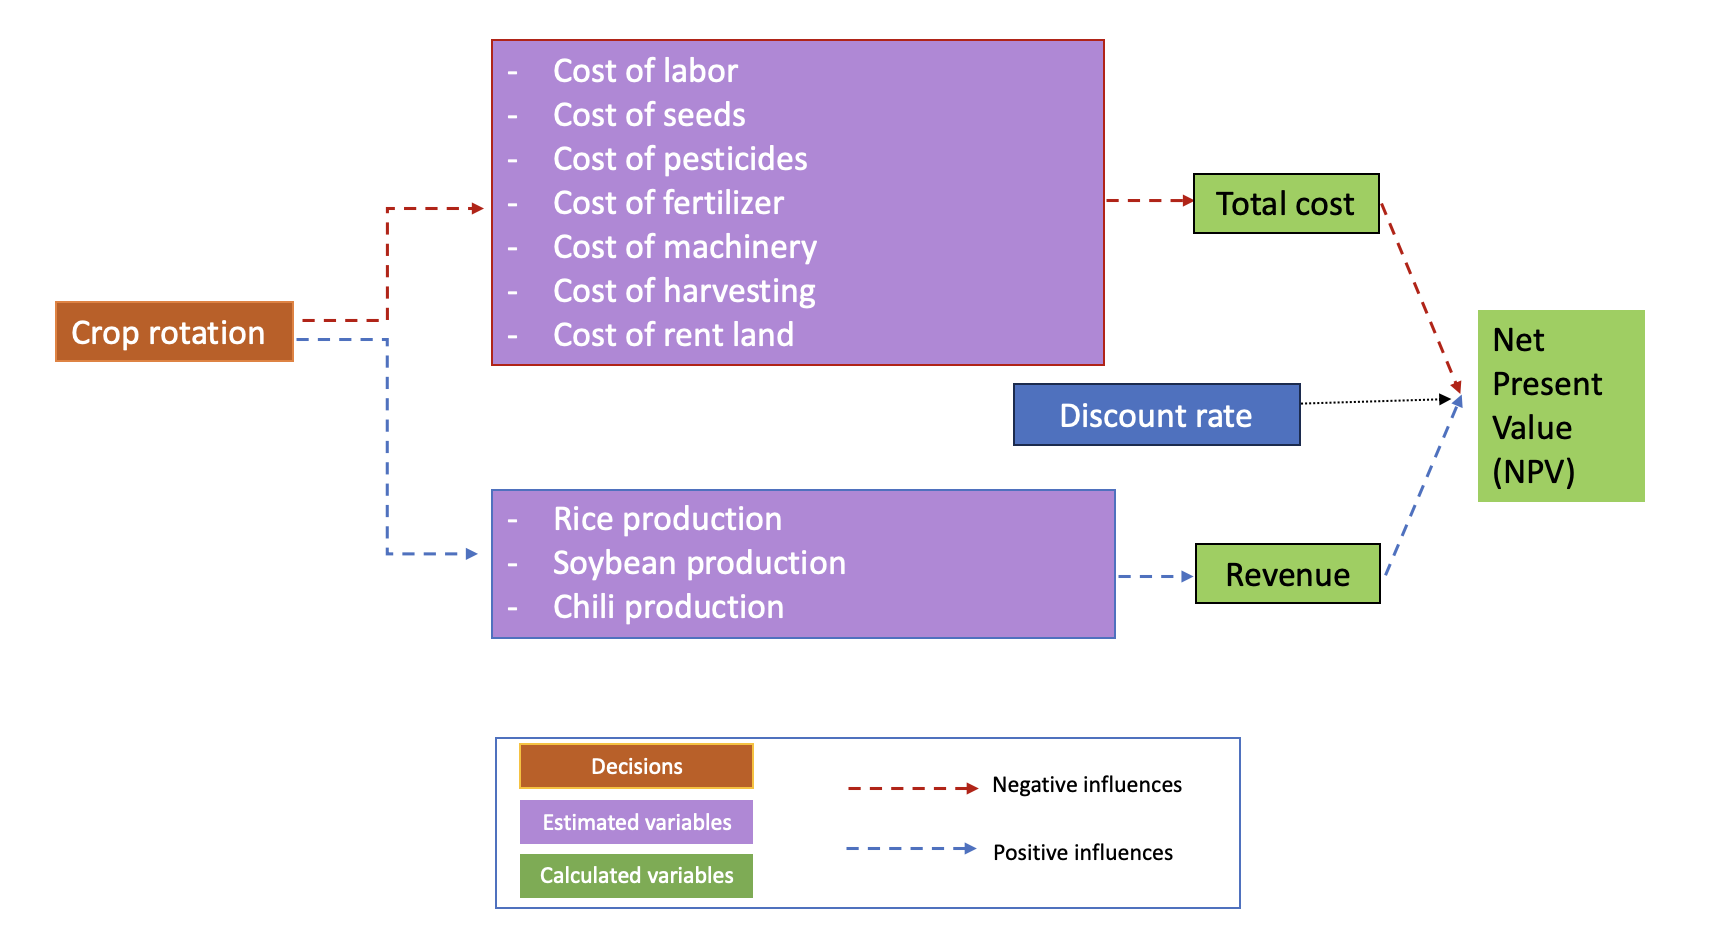
\includegraphics{Photo rice farm with crop rotation/conceptual model.png}

\hypertarget{variable-used-in-conceptual-model}{%
\subsubsection{Variable used in conceptual
model}\label{variable-used-in-conceptual-model}}

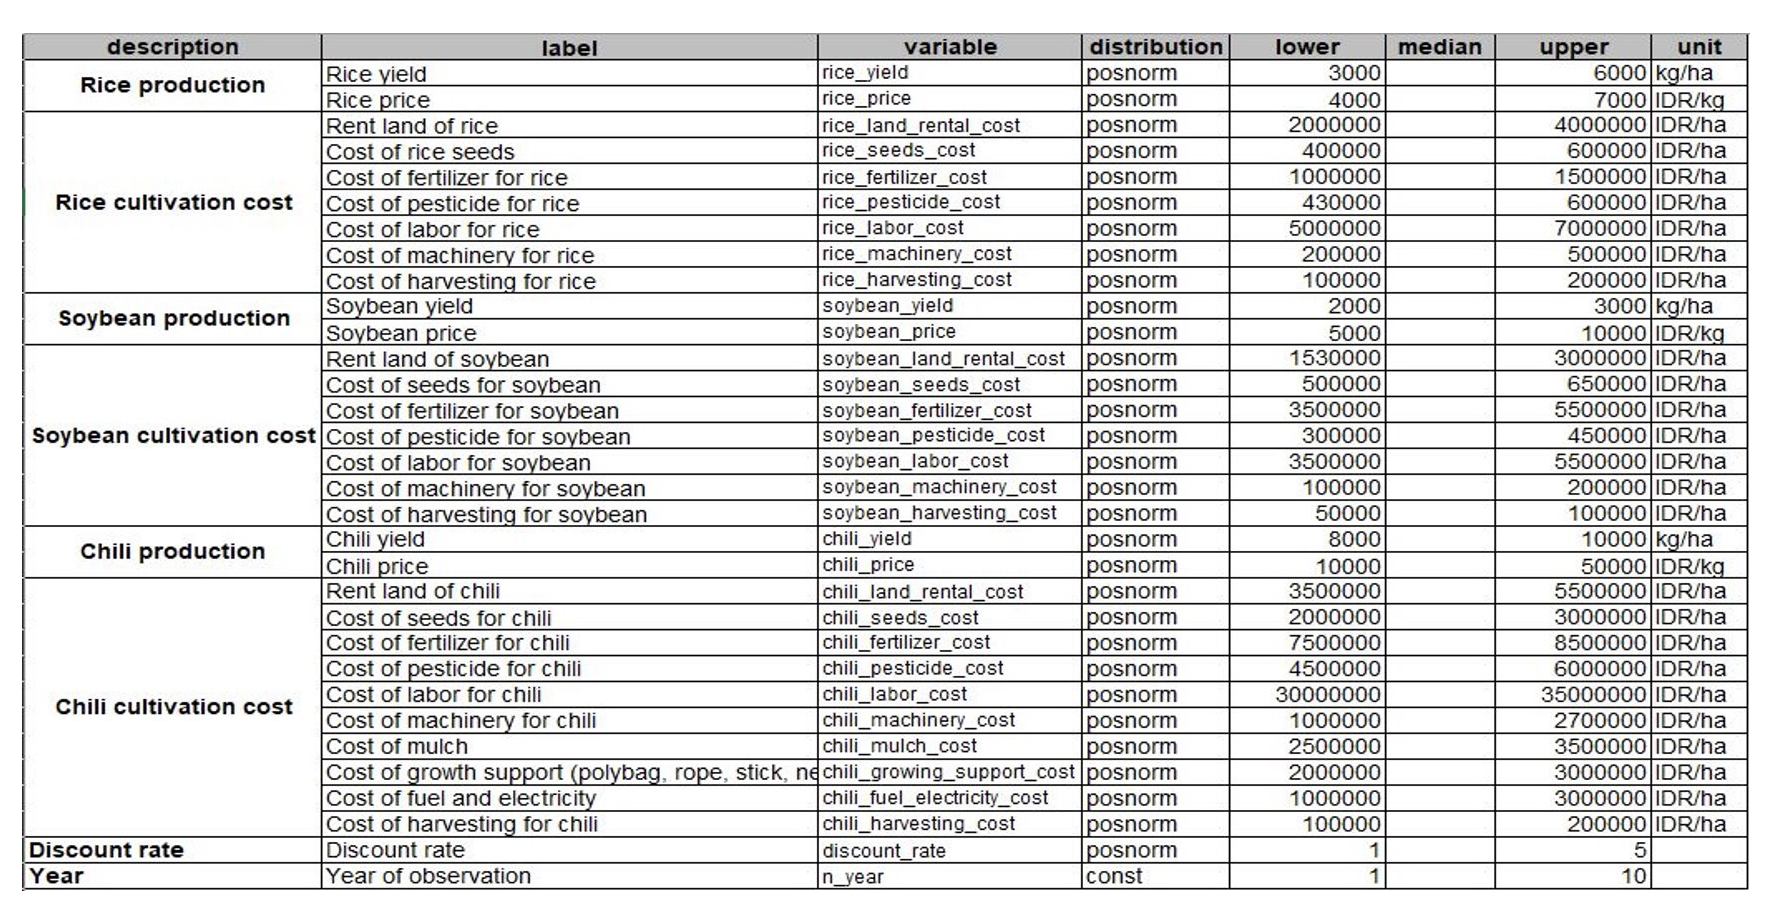
\includegraphics{Photo rice farm with crop rotation/Variable estimate.png}

Variable for rice farm and crop rotation for small holder farmers in
Indonesia have 8 mains variables that are consist of rice production,
rice cultivation cost, soybean production, soybean cultivation cost,
chili production, chili cultivation cost, discount rate and year of
system. Overall, there are 33 variables that are used for this decision
analysis.

\textbf{Source} :

BPS (2018), Mucharam et al. (2020), Jagung (2017), Fao (2018), BPS
(2022), Amirrullah (2019), Crystal and Whittlesey (2004), Jagung (2017),
BRIN (2022), USDA (2012), Setiartiti (2021), Antriyandarti (2015),
Krisdiana et al. (2021), Harsono et al. (2020), Schilling (1999),
Wandschneider et al. (2019), Sundari et al. (2021)

\hypertarget{estimate-calculation}{%
\subsection{Estimate Calculation}\label{estimate-calculation}}

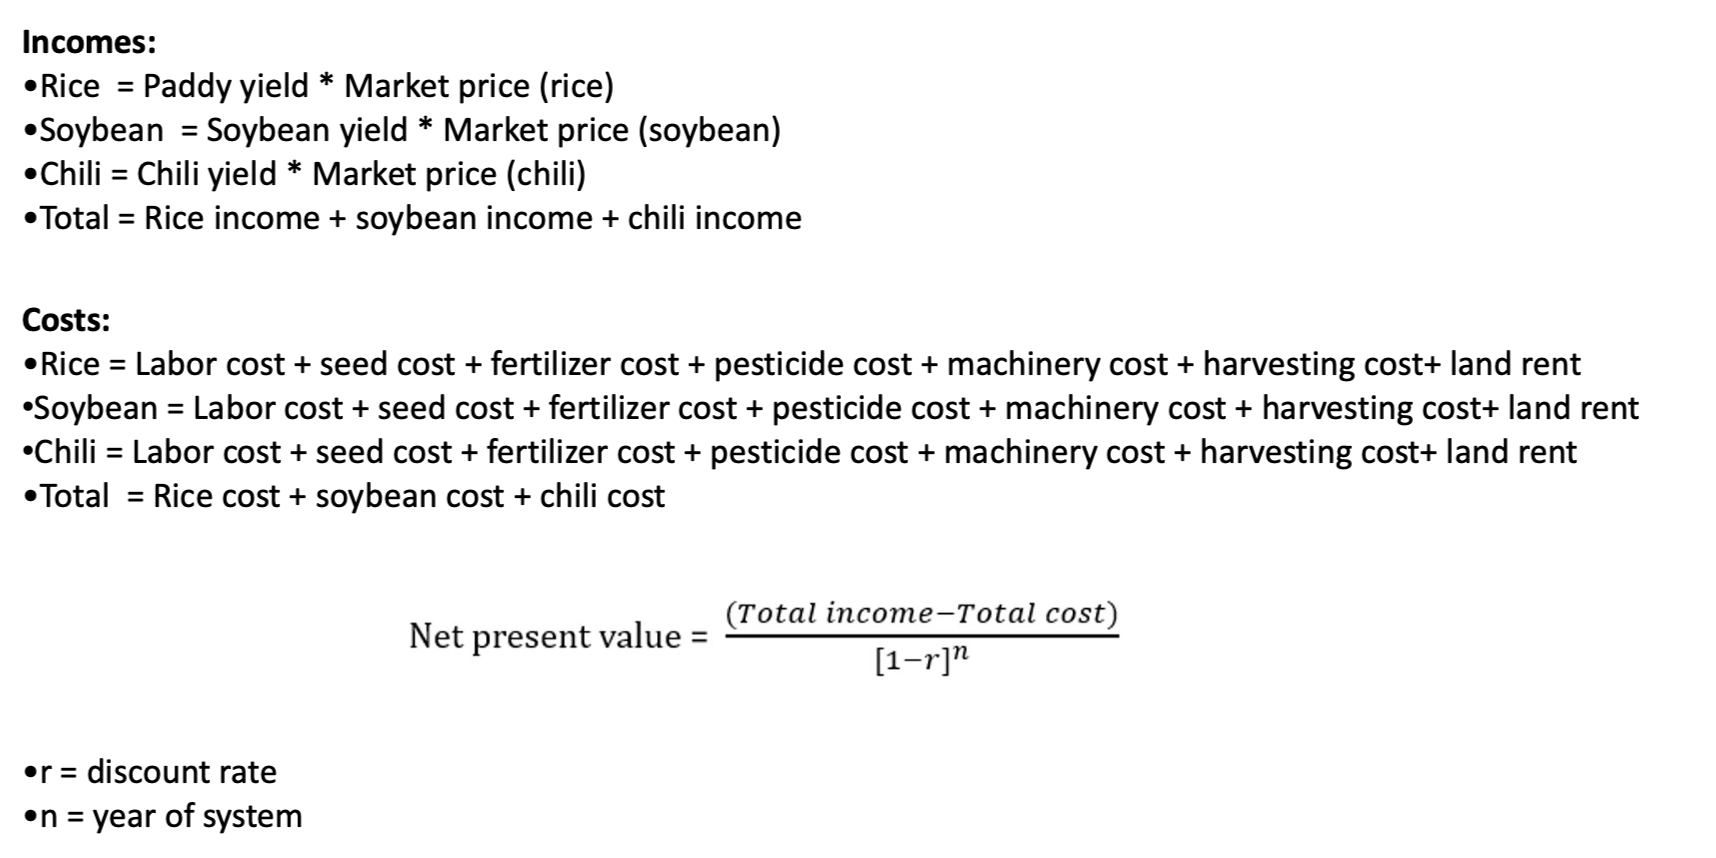
\includegraphics{Photo rice farm with crop rotation/Estimate calculation.png}
\textbf{NPV (Net Present Value)}: In financial terms, the NPV the
measurement of the profitability of a project or programme. This is
achieved by subtracting the current values of expenditure from the
current values of income over a period of time. Income can be referred
to as benefit and expenditure can be referred to as cost.

\textbf{Discount Rate}: The discount rate is the interest rate used in
analysis of discounted cash flow (DCF).

Stantec (2005)

\hypertarget{decision-analysis}{%
\subsection{Decision analysis}\label{decision-analysis}}

\hypertarget{r-code}{%
\subsubsection{R code}\label{r-code}}

Do, Luedeling, and Whitney (2020)

\begin{Shaded}
\begin{Highlighting}[]
\NormalTok{crop\_rotation\_decision }\OtherTok{\textless{}{-}} \ControlFlowTok{function}\NormalTok{()\{}
  
  \CommentTok{\# Estimate the income of rice in a normal season}
\NormalTok{  rice\_income }\OtherTok{\textless{}{-}} \FunctionTok{vv}\NormalTok{(rice\_yield }\SpecialCharTok{*}\NormalTok{ rice\_price, }\AttributeTok{n=}\NormalTok{n\_year, }\AttributeTok{var\_CV=}\DecValTok{100}\NormalTok{)}
  
  \CommentTok{\# Estimate the income of soybean in a normal season}
\NormalTok{  soybean\_income }\OtherTok{\textless{}{-}} \FunctionTok{vv}\NormalTok{(soybean\_yield }\SpecialCharTok{*}\NormalTok{ soybean\_price, }\AttributeTok{n=}\NormalTok{n\_year, }\AttributeTok{var\_CV=}\DecValTok{100}\NormalTok{)}
  
  \CommentTok{\# Estimate the income of chili in a normal season}
\NormalTok{  chili\_income }\OtherTok{\textless{}{-}} \FunctionTok{vv}\NormalTok{(chili\_yield }\SpecialCharTok{*}\NormalTok{ chili\_price, }\AttributeTok{n=}\NormalTok{n\_year, }\AttributeTok{var\_CV=}\DecValTok{100}\NormalTok{)}
  
  \CommentTok{\#Estimate the cost of rice farm in a normal season}
\NormalTok{  rice\_cost\_precal }\OtherTok{\textless{}{-}} \FunctionTok{sum}\NormalTok{(rice\_land\_rental\_cost, rice\_seeds\_cost, rice\_fertilizer\_cost,}
\NormalTok{                          rice\_pesticide\_cost, rice\_machinery\_cost, rice\_harvesting\_cost)}
\NormalTok{  rice\_cost }\OtherTok{\textless{}{-}} \FunctionTok{vv}\NormalTok{(rice\_cost\_precal, }\AttributeTok{n=}\NormalTok{n\_year, }\AttributeTok{var\_CV=}\DecValTok{100}\NormalTok{)}
  
  
  \CommentTok{\#Estimate the cost of soybean farm in a normal season}
\NormalTok{  soybean\_cost\_precal }\OtherTok{\textless{}{-}} \FunctionTok{sum}\NormalTok{(soybean\_land\_rental\_cost, soybean\_seeds\_cost, soybean\_fertilizer\_cost,}
\NormalTok{                             soybean\_pesticide\_cost, soybean\_machinery\_cost, soybean\_harvesting\_cost)}
\NormalTok{  soybean\_cost }\OtherTok{\textless{}{-}} \FunctionTok{vv}\NormalTok{(soybean\_cost\_precal, }\AttributeTok{n=}\NormalTok{n\_year, }\AttributeTok{var\_CV=}\DecValTok{100}\NormalTok{)}
  
  
  \CommentTok{\#Estimate the cost in a normal season}
\NormalTok{  chili\_cost\_precal }\OtherTok{\textless{}{-}} \FunctionTok{sum}\NormalTok{(chili\_land\_rental\_cost, chili\_seeds\_cost, chili\_fertilizer\_cost,}
\NormalTok{                           chili\_pesticide\_cost, chili\_machinery\_cost, chili\_harvesting\_cost)}
\NormalTok{  chili\_cost }\OtherTok{\textless{}{-}} \FunctionTok{vv}\NormalTok{(chili\_cost\_precal, }\AttributeTok{n=}\NormalTok{n\_year, }\AttributeTok{var\_CV=}\DecValTok{100}\NormalTok{)}
  
  
  \CommentTok{\# Estimate the profit}
\NormalTok{  rice\_profit }\OtherTok{\textless{}{-}} \FunctionTok{vv}\NormalTok{(rice\_income }\SpecialCharTok{{-}}\NormalTok{ rice\_cost, }\AttributeTok{n=}\NormalTok{n\_year, }\AttributeTok{var\_CV=}\DecValTok{100}\NormalTok{)}
\NormalTok{  soybean\_profit }\OtherTok{\textless{}{-}} \FunctionTok{vv}\NormalTok{(soybean\_income }\SpecialCharTok{{-}}\NormalTok{ soybean\_cost, }\AttributeTok{n=}\NormalTok{n\_year, }\AttributeTok{var\_CV=}\DecValTok{100}\NormalTok{)}
\NormalTok{  chili\_profit }\OtherTok{\textless{}{-}} \FunctionTok{vv}\NormalTok{(chili\_income }\SpecialCharTok{{-}}\NormalTok{ chili\_cost, }\AttributeTok{n=}\NormalTok{n\_year, }\AttributeTok{var\_CV=}\DecValTok{100}\NormalTok{)}
  
  
  \CommentTok{\# Final result}
  \CommentTok{\#assuming rice cultivation is 3 times per year  }
\NormalTok{  rice\_cultivation\_result }\OtherTok{=} \FunctionTok{vv}\NormalTok{(rice\_profit}\SpecialCharTok{*}\DecValTok{3}\NormalTok{, }\AttributeTok{n=}\NormalTok{n\_year, }\AttributeTok{var\_CV=}\DecValTok{100}\NormalTok{)}
  
  \CommentTok{\#crop rotation decision scenario}
  \CommentTok{\#if crop rotation of 3 crops is done in one year}
\NormalTok{  crop\_rotation\_result }\OtherTok{=} \FunctionTok{vv}\NormalTok{(rice\_profit }\SpecialCharTok{+}\NormalTok{ soybean\_profit }\SpecialCharTok{+}\NormalTok{ chili\_profit, }\AttributeTok{n=}\NormalTok{n\_year, }\AttributeTok{var\_CV=}\DecValTok{100}\NormalTok{)}
  
  \CommentTok{\#if crop rotation of rice and soybean is done in one year (rice{-}soybean{-}rice)}
\NormalTok{  rice\_soybean\_result }\OtherTok{=} \FunctionTok{vv}\NormalTok{((rice\_profit}\SpecialCharTok{*}\DecValTok{2}\NormalTok{) }\SpecialCharTok{+}\NormalTok{ soybean\_profit, }\AttributeTok{n=}\NormalTok{n\_year, }\AttributeTok{var\_CV=}\DecValTok{100}\NormalTok{)}
  
  \CommentTok{\#if crop rotation of rice and chili is done in one year (rice{-}chili)}
\NormalTok{  rice\_chili\_result }\OtherTok{=} \FunctionTok{vv}\NormalTok{(rice\_profit }\SpecialCharTok{+}\NormalTok{ chili\_profit, }\AttributeTok{n=}\NormalTok{n\_year, }\AttributeTok{var\_CV=}\DecValTok{100}\NormalTok{)}
  
  
  \CommentTok{\# NPV}
\NormalTok{  NPV\_rice }\OtherTok{\textless{}{-}} \FunctionTok{discount}\NormalTok{(rice\_cultivation\_result, discount\_rate, }\AttributeTok{calculate\_NPV =} \ConstantTok{TRUE}\NormalTok{)}
\NormalTok{  NPV\_crop\_rotation }\OtherTok{\textless{}{-}} \FunctionTok{discount}\NormalTok{(crop\_rotation\_result, discount\_rate, }\AttributeTok{calculate\_NPV =} \ConstantTok{TRUE}\NormalTok{)}
\NormalTok{  NPV\_rice\_soybean }\OtherTok{\textless{}{-}} \FunctionTok{discount}\NormalTok{(rice\_soybean\_result, discount\_rate, }\AttributeTok{calculate\_NPV =} \ConstantTok{TRUE}\NormalTok{)}
\NormalTok{  NPV\_rice\_chili }\OtherTok{\textless{}{-}} \FunctionTok{discount}\NormalTok{(rice\_chili\_result, discount\_rate, }\AttributeTok{calculate\_NPV =} \ConstantTok{TRUE}\NormalTok{)}
  
  
  \CommentTok{\# Cashflow}
\NormalTok{  cashflow\_crop\_rotation }\OtherTok{\textless{}{-}}\NormalTok{ crop\_rotation\_result }\SpecialCharTok{{-}}\NormalTok{ rice\_cultivation\_result}
\NormalTok{  cashflow\_rice\_soybean }\OtherTok{\textless{}{-}}\NormalTok{ rice\_soybean\_result }\SpecialCharTok{{-}}\NormalTok{ rice\_cultivation\_result}
\NormalTok{  cashflow\_rice\_chili }\OtherTok{\textless{}{-}}\NormalTok{ rice\_chili\_result }\SpecialCharTok{{-}}\NormalTok{ rice\_cultivation\_result}
  
  
  \CommentTok{\# Generate the list of outputs from the Monte Carlo simulation}
  \FunctionTok{return}\NormalTok{(}\FunctionTok{list}\NormalTok{(}\AttributeTok{Rice\_NPV =}\NormalTok{ NPV\_rice,}
              \AttributeTok{crop\_rotation\_NPV =}\NormalTok{ NPV\_crop\_rotation,}
              \AttributeTok{rice\_soybean\_NPV =}\NormalTok{ NPV\_rice\_soybean,}
              \AttributeTok{rice\_chili\_NPV=}\NormalTok{ NPV\_rice\_chili,}
              \AttributeTok{NPV\_decision\_crop\_rotation =}\NormalTok{ NPV\_crop\_rotation }\SpecialCharTok{{-}}\NormalTok{ NPV\_rice,}
              \AttributeTok{NPV\_decision\_rice\_soybean =}\NormalTok{ NPV\_rice\_soybean }\SpecialCharTok{{-}}\NormalTok{ NPV\_rice,}
              \AttributeTok{NPV\_decision\_rice\_chili =}\NormalTok{ NPV\_rice\_chili }\SpecialCharTok{{-}}\NormalTok{ NPV\_rice,}
              \AttributeTok{cashflow\_crop\_rotation =}\NormalTok{ cashflow\_crop\_rotation,}
              \AttributeTok{cashflow\_rice\_soybean =}\NormalTok{ cashflow\_rice\_soybean,}
              \AttributeTok{cashflow\_rice\_chili =}\NormalTok{ cashflow\_rice\_chili}
\NormalTok{  ))}
\NormalTok{\}}

\CommentTok{\# Run the Monte Carlo simulation using the model function}
\NormalTok{input\_estimates }\OtherTok{\textless{}{-}} \FunctionTok{read.csv}\NormalTok{(}\StringTok{"new\_variable\_estimates.csv"}\NormalTok{, }\AttributeTok{sep=}\StringTok{";"}\NormalTok{)}

\NormalTok{crop\_rotation\_mc\_simulation }\OtherTok{\textless{}{-}} \FunctionTok{mcSimulation}\NormalTok{(}\AttributeTok{estimate =} \FunctionTok{as.estimate}\NormalTok{(input\_estimates),}
                                            \AttributeTok{model\_function =}\NormalTok{ crop\_rotation\_decision,}
                                            \AttributeTok{numberOfModelRuns =} \DecValTok{1000}\NormalTok{,}
                                            \AttributeTok{functionSyntax =} \StringTok{"plainNames"}\NormalTok{)}

\CommentTok{\# Run the Monte Carlo simulation using the model function}
\NormalTok{input\_estimates }\OtherTok{\textless{}{-}} \FunctionTok{read.csv}\NormalTok{(}\StringTok{"new\_variable\_estimates.csv"}\NormalTok{, }\AttributeTok{sep=}\StringTok{";"}\NormalTok{)}

\NormalTok{crop\_rotation\_mc\_simulation }\OtherTok{\textless{}{-}} \FunctionTok{mcSimulation}\NormalTok{(}\AttributeTok{estimate =} \FunctionTok{as.estimate}\NormalTok{(input\_estimates),}
                                            \AttributeTok{model\_function =}\NormalTok{ crop\_rotation\_decision,}
                                            \AttributeTok{numberOfModelRuns =} \DecValTok{1000}\NormalTok{,}
                                            \AttributeTok{functionSyntax =} \StringTok{"plainNames"}\NormalTok{)}
\end{Highlighting}
\end{Shaded}

\hypertarget{plot-npv-distribution-analysis}{%
\subsubsection{Plot NPV distribution
analysis}\label{plot-npv-distribution-analysis}}

\hypertarget{npv-for-crop-rotation-rice-soybean-chili}{%
\paragraph{NPV for crop rotation
(rice-soybean-chili)}\label{npv-for-crop-rotation-rice-soybean-chili}}

\begin{Shaded}
\begin{Highlighting}[]
\NormalTok{decisionSupport}\SpecialCharTok{::}\FunctionTok{plot\_distributions}\NormalTok{(}\AttributeTok{mcSimulation\_object =}\NormalTok{ crop\_rotation\_mc\_simulation, }
                                    \AttributeTok{vars =} \FunctionTok{c}\NormalTok{(}\StringTok{"crop\_rotation\_NPV"}\NormalTok{, }\StringTok{"Rice\_NPV"}\NormalTok{),}
                                    \AttributeTok{method =} \StringTok{\textquotesingle{}smooth\_simple\_overlay\textquotesingle{}}\NormalTok{)}
\end{Highlighting}
\end{Shaded}

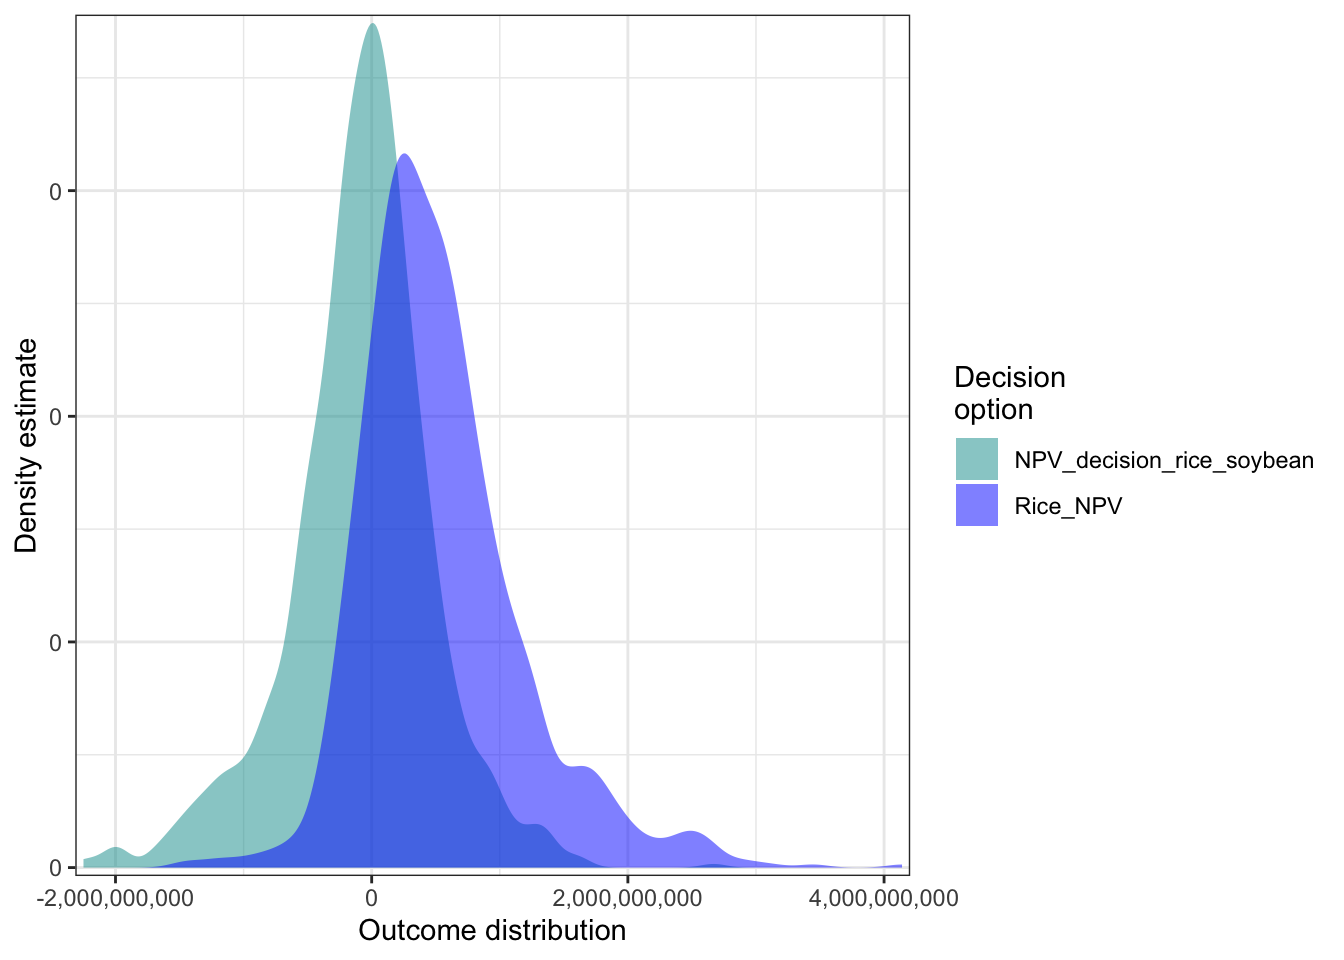
\includegraphics{Rice-farm-with-crop-rotation_files/figure-latex/unnamed-chunk-8-1.pdf}

\begin{Shaded}
\begin{Highlighting}[]
\NormalTok{decisionSupport}\SpecialCharTok{::}\FunctionTok{plot\_distributions}\NormalTok{(}\AttributeTok{mcSimulation\_object =}\NormalTok{ crop\_rotation\_mc\_simulation, }
                                    \AttributeTok{vars =} \FunctionTok{c}\NormalTok{(}\StringTok{"crop\_rotation\_NPV"}\NormalTok{, }\StringTok{"Rice\_NPV"}\NormalTok{),}
                                    \AttributeTok{method =} \StringTok{\textquotesingle{}boxplot\textquotesingle{}}\NormalTok{)}
\end{Highlighting}
\end{Shaded}

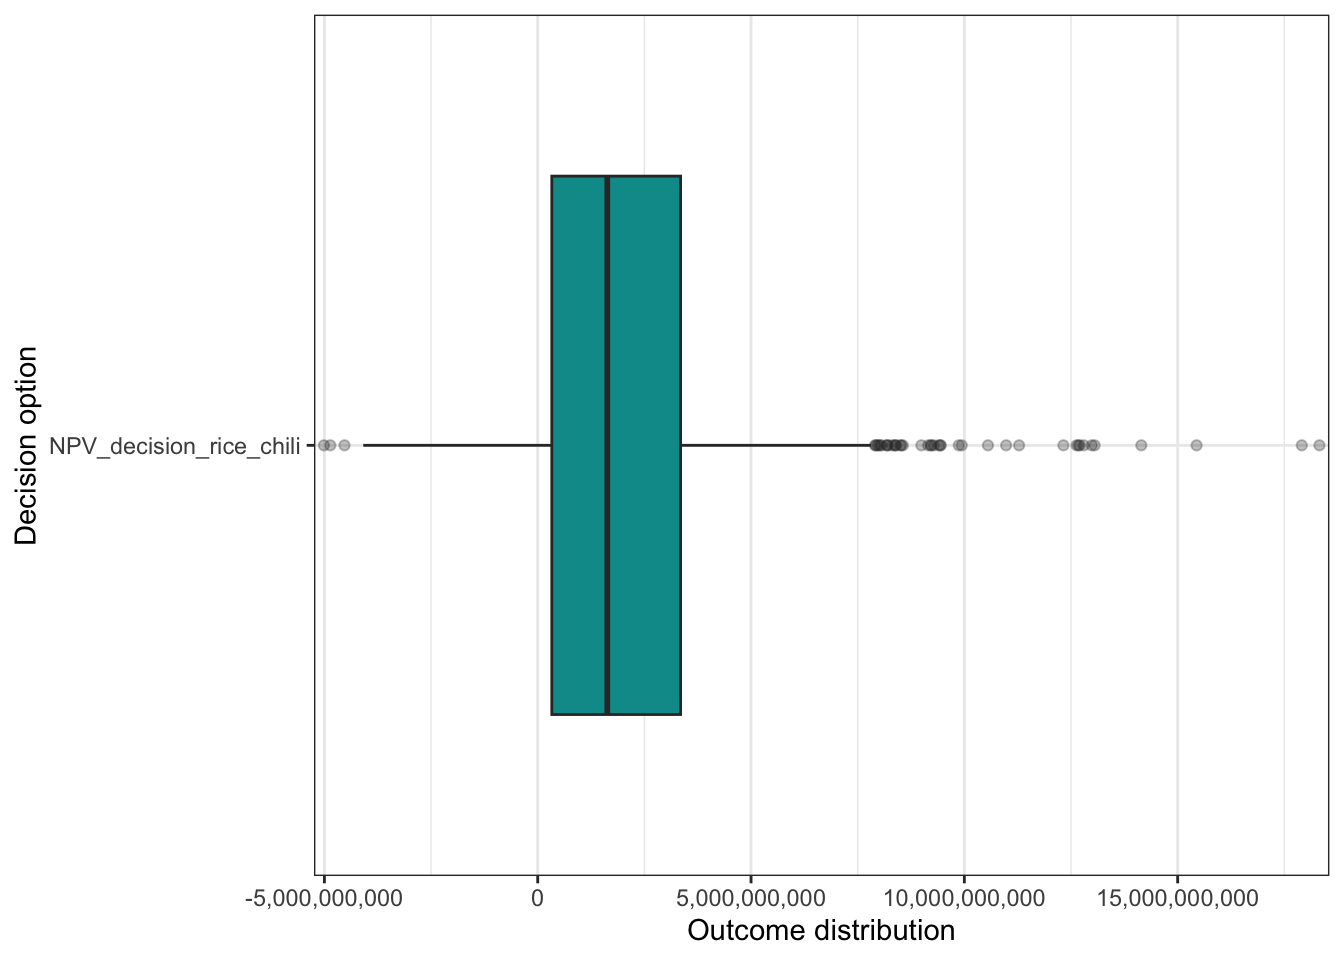
\includegraphics{Rice-farm-with-crop-rotation_files/figure-latex/unnamed-chunk-8-2.pdf}

\begin{Shaded}
\begin{Highlighting}[]
\NormalTok{decisionSupport}\SpecialCharTok{::}\FunctionTok{plot\_distributions}\NormalTok{(}\AttributeTok{mcSimulation\_object =}\NormalTok{ crop\_rotation\_mc\_simulation, }
                                    \AttributeTok{vars =} \FunctionTok{c}\NormalTok{(}\StringTok{"NPV\_decision\_crop\_rotation"}\NormalTok{),}
                                    \AttributeTok{method =} \StringTok{\textquotesingle{}boxplot\_density\textquotesingle{}}\NormalTok{)}
\end{Highlighting}
\end{Shaded}

\begin{verbatim}
## Warning: The following aesthetics were dropped during statistical transformation: x
## i This can happen when ggplot fails to infer the correct grouping structure in
##   the data.
## i Did you forget to specify a `group` aesthetic or to convert a numerical
##   variable into a factor?
\end{verbatim}

\includegraphics{Rice-farm-with-crop-rotation_files/figure-latex/unnamed-chunk-8-3.pdf}

\hypertarget{npv-for-crop-rotation-rice-soybean-rice}{%
\paragraph{NPV for crop rotation
(rice-soybean-rice)}\label{npv-for-crop-rotation-rice-soybean-rice}}

\begin{Shaded}
\begin{Highlighting}[]
\NormalTok{decisionSupport}\SpecialCharTok{::}\FunctionTok{plot\_distributions}\NormalTok{(}\AttributeTok{mcSimulation\_object =}\NormalTok{ crop\_rotation\_mc\_simulation, }
                                    \AttributeTok{vars =} \FunctionTok{c}\NormalTok{(}\StringTok{"rice\_soybean\_NPV"}\NormalTok{,}\StringTok{"Rice\_NPV"}\NormalTok{),}
                                    \AttributeTok{method =} \StringTok{\textquotesingle{}smooth\_simple\_overlay\textquotesingle{}}\NormalTok{)}
\end{Highlighting}
\end{Shaded}

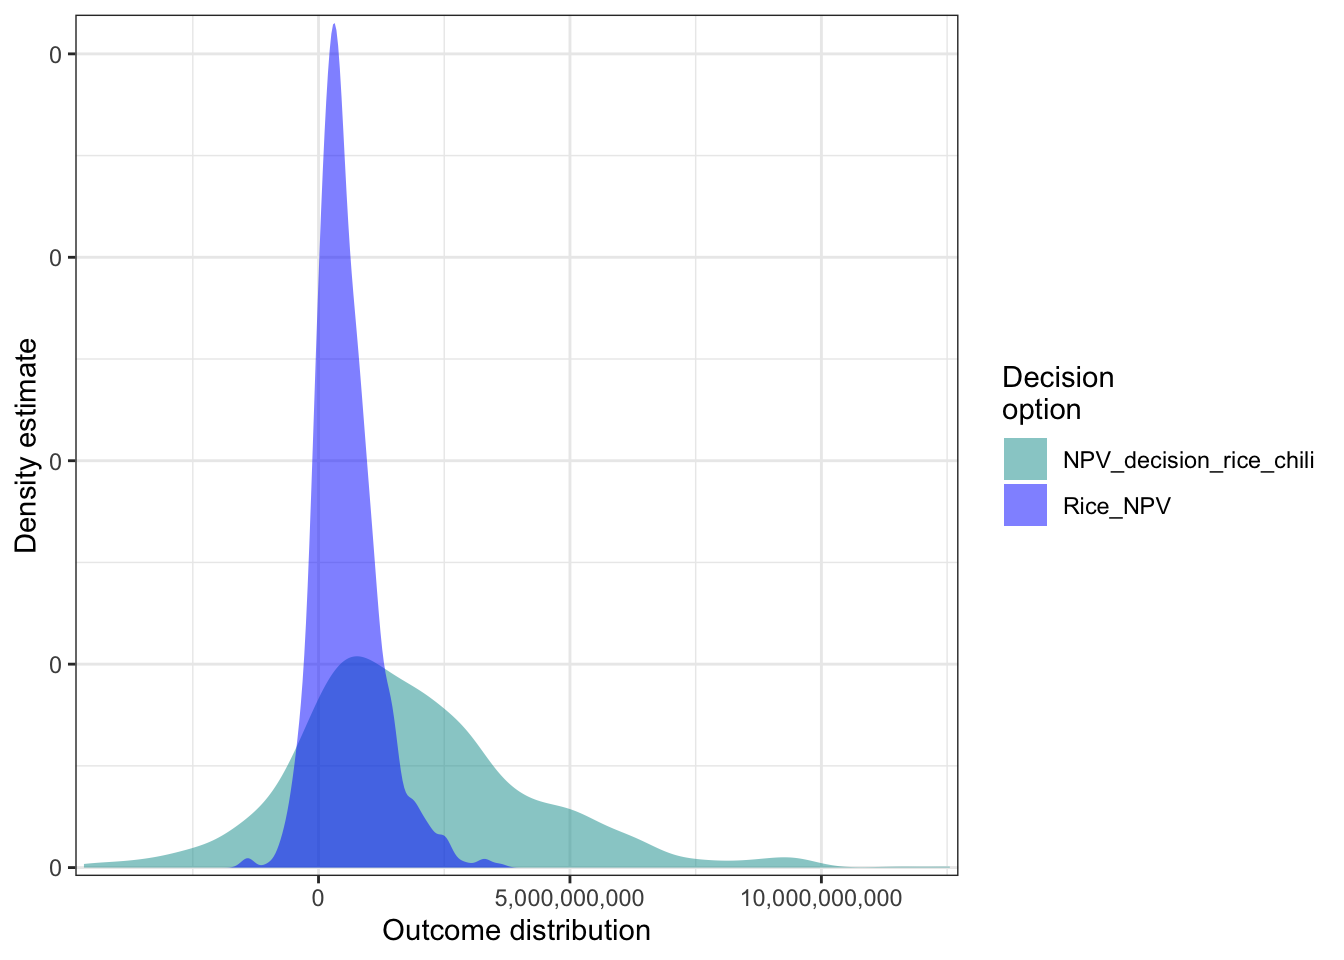
\includegraphics{Rice-farm-with-crop-rotation_files/figure-latex/unnamed-chunk-9-1.pdf}

\begin{Shaded}
\begin{Highlighting}[]
\NormalTok{decisionSupport}\SpecialCharTok{::}\FunctionTok{plot\_distributions}\NormalTok{(}\AttributeTok{mcSimulation\_object =}\NormalTok{ crop\_rotation\_mc\_simulation, }
                                    \AttributeTok{vars =} \FunctionTok{c}\NormalTok{(}\StringTok{"rice\_soybean\_NPV"}\NormalTok{,}\StringTok{"Rice\_NPV"}\NormalTok{),}
                                    \AttributeTok{method =} \StringTok{\textquotesingle{}boxplot\textquotesingle{}}\NormalTok{)}
\end{Highlighting}
\end{Shaded}

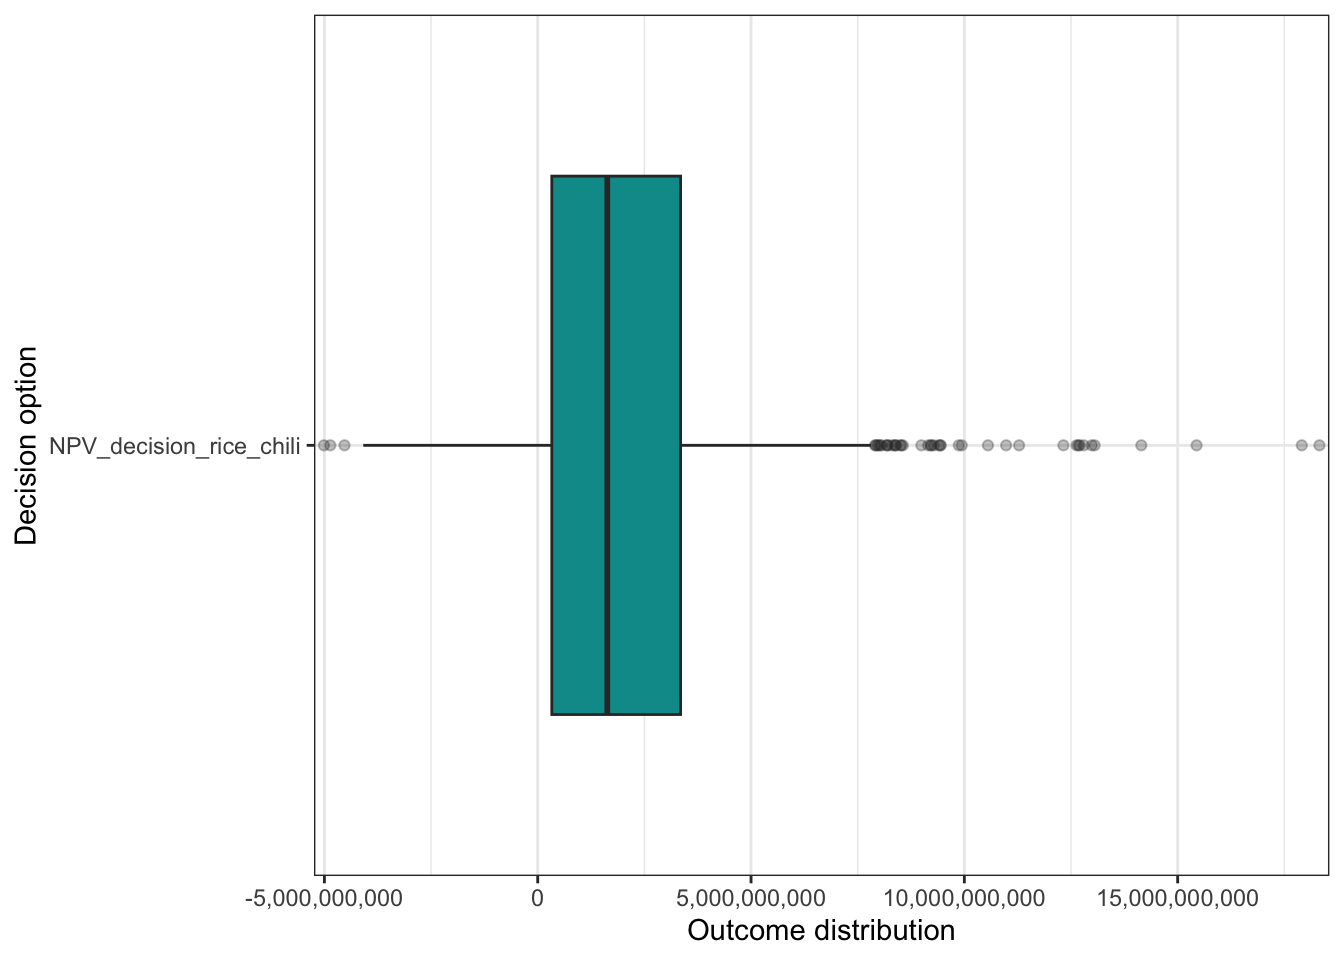
\includegraphics{Rice-farm-with-crop-rotation_files/figure-latex/unnamed-chunk-9-2.pdf}

\begin{Shaded}
\begin{Highlighting}[]
\NormalTok{decisionSupport}\SpecialCharTok{::}\FunctionTok{plot\_distributions}\NormalTok{(}\AttributeTok{mcSimulation\_object =}\NormalTok{ crop\_rotation\_mc\_simulation, }
                                    \AttributeTok{vars =} \FunctionTok{c}\NormalTok{(}\StringTok{"NPV\_decision\_rice\_soybean"}\NormalTok{),}
                                    \AttributeTok{method =} \StringTok{\textquotesingle{}boxplot\_density\textquotesingle{}}\NormalTok{)}
\end{Highlighting}
\end{Shaded}

\begin{verbatim}
## Warning: The following aesthetics were dropped during statistical transformation: x
## i This can happen when ggplot fails to infer the correct grouping structure in
##   the data.
## i Did you forget to specify a `group` aesthetic or to convert a numerical
##   variable into a factor?
\end{verbatim}

\includegraphics{Rice-farm-with-crop-rotation_files/figure-latex/unnamed-chunk-9-3.pdf}

\hypertarget{npv-for-crop-rotation-rice-chilli}{%
\paragraph{NPV for crop rotation
(rice-chilli)}\label{npv-for-crop-rotation-rice-chilli}}

\begin{Shaded}
\begin{Highlighting}[]
\NormalTok{decisionSupport}\SpecialCharTok{::}\FunctionTok{plot\_distributions}\NormalTok{(}\AttributeTok{mcSimulation\_object =}\NormalTok{ crop\_rotation\_mc\_simulation, }
                                    \AttributeTok{vars =} \FunctionTok{c}\NormalTok{(}\StringTok{"rice\_chili\_NPV"}\NormalTok{,}\StringTok{"Rice\_NPV"}\NormalTok{),}
                                    \AttributeTok{method =} \StringTok{\textquotesingle{}smooth\_simple\_overlay\textquotesingle{}}\NormalTok{)}
\end{Highlighting}
\end{Shaded}

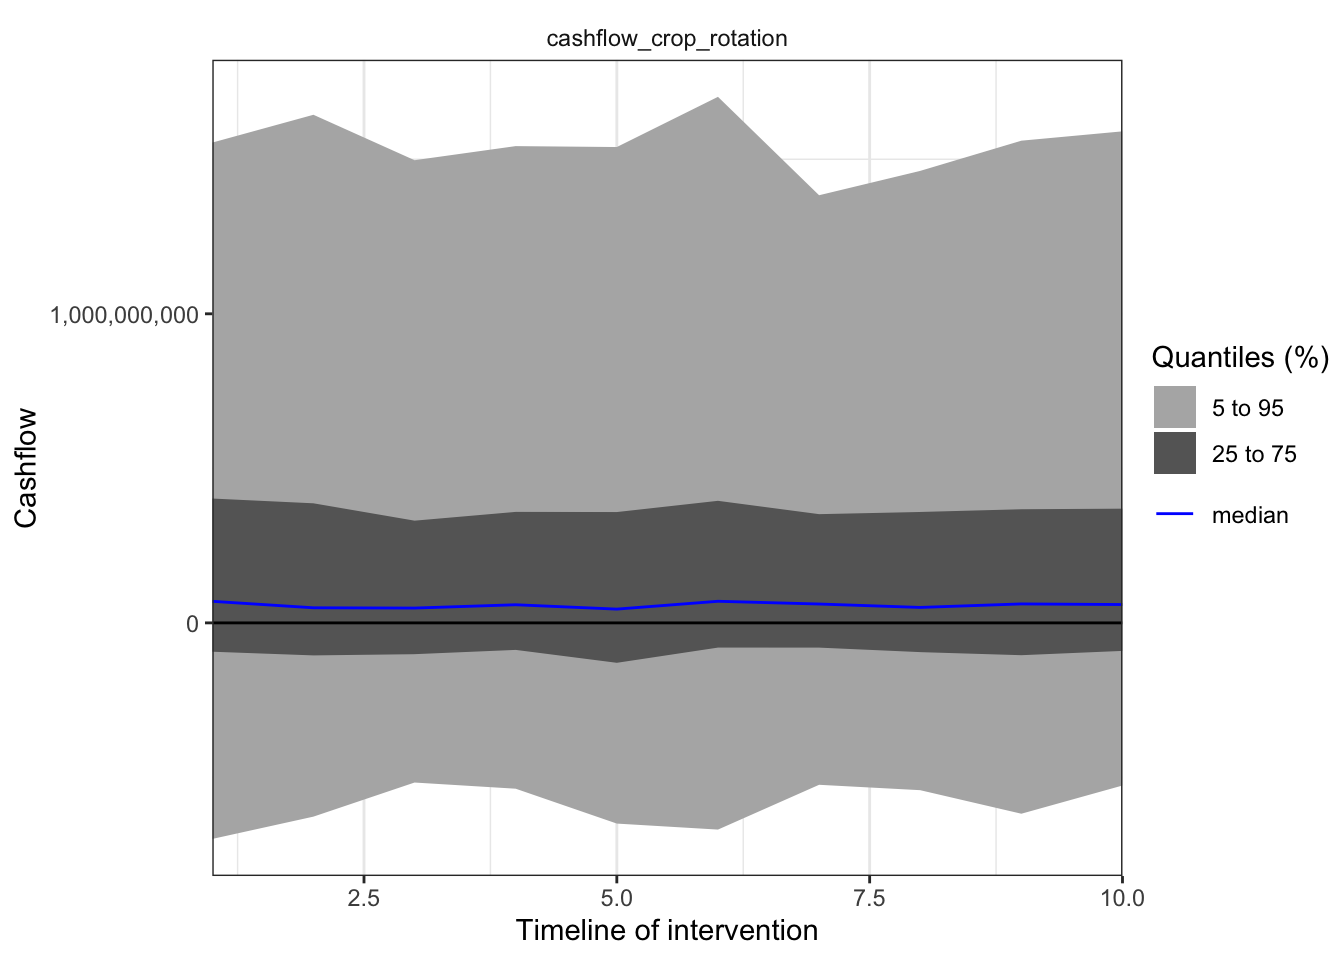
\includegraphics{Rice-farm-with-crop-rotation_files/figure-latex/unnamed-chunk-10-1.pdf}

\begin{Shaded}
\begin{Highlighting}[]
\NormalTok{decisionSupport}\SpecialCharTok{::}\FunctionTok{plot\_distributions}\NormalTok{(}\AttributeTok{mcSimulation\_object =}\NormalTok{ crop\_rotation\_mc\_simulation, }
                                    \AttributeTok{vars =} \FunctionTok{c}\NormalTok{(}\StringTok{"rice\_chili\_NPV"}\NormalTok{,}\StringTok{"Rice\_NPV"}\NormalTok{),}
                                    \AttributeTok{method =} \StringTok{\textquotesingle{}boxplot\textquotesingle{}}\NormalTok{)}
\end{Highlighting}
\end{Shaded}

\includegraphics{Rice-farm-with-crop-rotation_files/figure-latex/unnamed-chunk-10-2.pdf}

\begin{Shaded}
\begin{Highlighting}[]
\NormalTok{decisionSupport}\SpecialCharTok{::}\FunctionTok{plot\_distributions}\NormalTok{(}\AttributeTok{mcSimulation\_object =}\NormalTok{ crop\_rotation\_mc\_simulation, }
                                    \AttributeTok{vars =} \FunctionTok{c}\NormalTok{(}\StringTok{"NPV\_decision\_rice\_chili"}\NormalTok{),}
                                    \AttributeTok{method =} \StringTok{\textquotesingle{}boxplot\_density\textquotesingle{}}\NormalTok{)}
\end{Highlighting}
\end{Shaded}

\begin{verbatim}
## Warning: The following aesthetics were dropped during statistical transformation: x
## i This can happen when ggplot fails to infer the correct grouping structure in
##   the data.
## i Did you forget to specify a `group` aesthetic or to convert a numerical
##   variable into a factor?
\end{verbatim}

\includegraphics{Rice-farm-with-crop-rotation_files/figure-latex/unnamed-chunk-10-3.pdf}

\hypertarget{cashflow-analysis}{%
\subsubsection{Cashflow analysis}\label{cashflow-analysis}}

\hypertarget{with-crop-rotation-of-3-crops-rice-soybean-chili}{%
\paragraph{With crop rotation of 3 crops
(rice-soybean-chili)}\label{with-crop-rotation-of-3-crops-rice-soybean-chili}}

\begin{Shaded}
\begin{Highlighting}[]
\FunctionTok{plot\_cashflow}\NormalTok{(}\AttributeTok{mcSimulation\_object =}\NormalTok{ crop\_rotation\_mc\_simulation, }\AttributeTok{cashflow\_var\_name =} \StringTok{"cashflow\_crop\_rotation"}\NormalTok{)}
\end{Highlighting}
\end{Shaded}

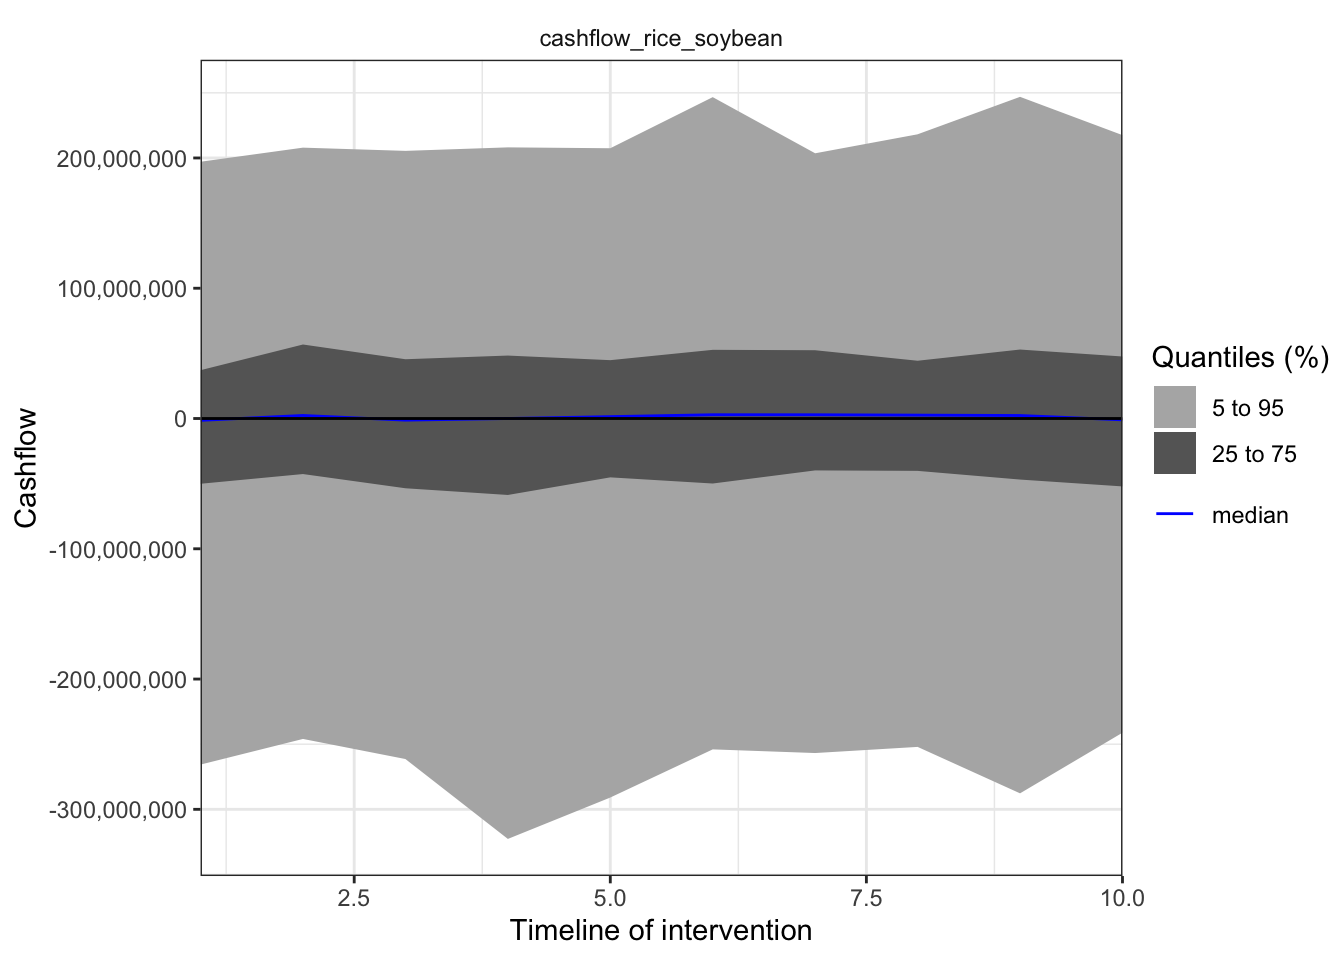
\includegraphics{Rice-farm-with-crop-rotation_files/figure-latex/unnamed-chunk-11-1.pdf}

\hypertarget{with-crop-rotation-of-rice-and-soybean-rice-soybean-rice}{%
\paragraph{With crop rotation of rice and soybean
(rice-soybean-rice)}\label{with-crop-rotation-of-rice-and-soybean-rice-soybean-rice}}

\begin{Shaded}
\begin{Highlighting}[]
\FunctionTok{plot\_cashflow}\NormalTok{(}\AttributeTok{mcSimulation\_object =}\NormalTok{ crop\_rotation\_mc\_simulation, }\AttributeTok{cashflow\_var\_name =} \StringTok{"cashflow\_rice\_soybean"}\NormalTok{)}
\end{Highlighting}
\end{Shaded}

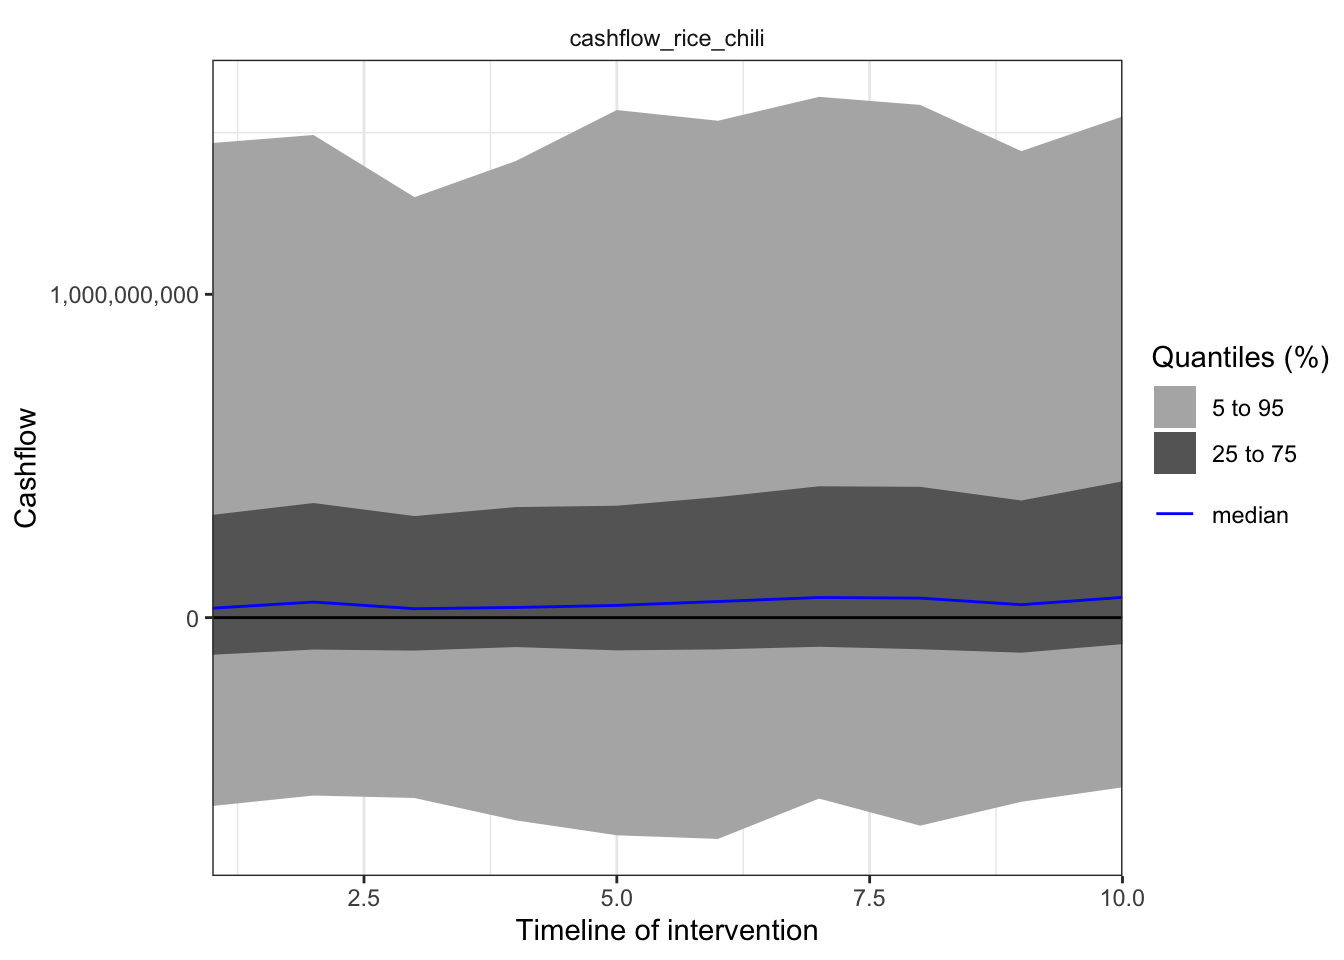
\includegraphics{Rice-farm-with-crop-rotation_files/figure-latex/unnamed-chunk-12-1.pdf}

\hypertarget{with-crop-rotation-of-rice-and-chili-rice-chili}{%
\paragraph{With crop rotation of rice and chili
(rice-chili)}\label{with-crop-rotation-of-rice-and-chili-rice-chili}}

\begin{Shaded}
\begin{Highlighting}[]
\FunctionTok{plot\_cashflow}\NormalTok{(}\AttributeTok{mcSimulation\_object =}\NormalTok{ crop\_rotation\_mc\_simulation, }\AttributeTok{cashflow\_var\_name =} \StringTok{"cashflow\_rice\_chili"}\NormalTok{)}
\end{Highlighting}
\end{Shaded}

\includegraphics{Rice-farm-with-crop-rotation_files/figure-latex/unnamed-chunk-13-1.pdf}

\hypertarget{value-of-information-voi-analysis}{%
\subsubsection{Value of Information (VoI)
analysis}\label{value-of-information-voi-analysis}}

\begin{Shaded}
\begin{Highlighting}[]
\NormalTok{mcSimulation\_table }\OtherTok{\textless{}{-}} \FunctionTok{data.frame}\NormalTok{(crop\_rotation\_mc\_simulation}\SpecialCharTok{$}\NormalTok{x, crop\_rotation\_mc\_simulation}\SpecialCharTok{$}\NormalTok{y[}\DecValTok{1}\SpecialCharTok{:}\DecValTok{7}\NormalTok{])}
\end{Highlighting}
\end{Shaded}

\hypertarget{evpi-crop-rotation}{%
\paragraph{EVPI crop rotation}\label{evpi-crop-rotation}}

\begin{Shaded}
\begin{Highlighting}[]
\NormalTok{evpi\_crop\_rotation }\OtherTok{\textless{}{-}} \FunctionTok{multi\_EVPI}\NormalTok{(}\AttributeTok{mc =}\NormalTok{ mcSimulation\_table, }\AttributeTok{first\_out\_var =} \StringTok{"crop\_rotation\_NPV"}\NormalTok{)}
\end{Highlighting}
\end{Shaded}

\begin{verbatim}
## [1] "Processing 6 output variables. This can take some time."
## [1] "Output variable 1 (crop_rotation_NPV) completed."
## [1] "Output variable 2 (rice_soybean_NPV) completed."
## [1] "Output variable 3 (rice_chili_NPV) completed."
## [1] "Output variable 4 (NPV_decision_crop_rotation) completed."
## [1] "Output variable 5 (NPV_decision_rice_soybean) completed."
## [1] "Output variable 6 (NPV_decision_rice_chili) completed."
\end{verbatim}

\begin{Shaded}
\begin{Highlighting}[]
\FunctionTok{plot\_evpi}\NormalTok{(evpi\_crop\_rotation, }\AttributeTok{decision\_vars =} \StringTok{"NPV\_decision\_crop\_rotation"}\NormalTok{)}
\end{Highlighting}
\end{Shaded}

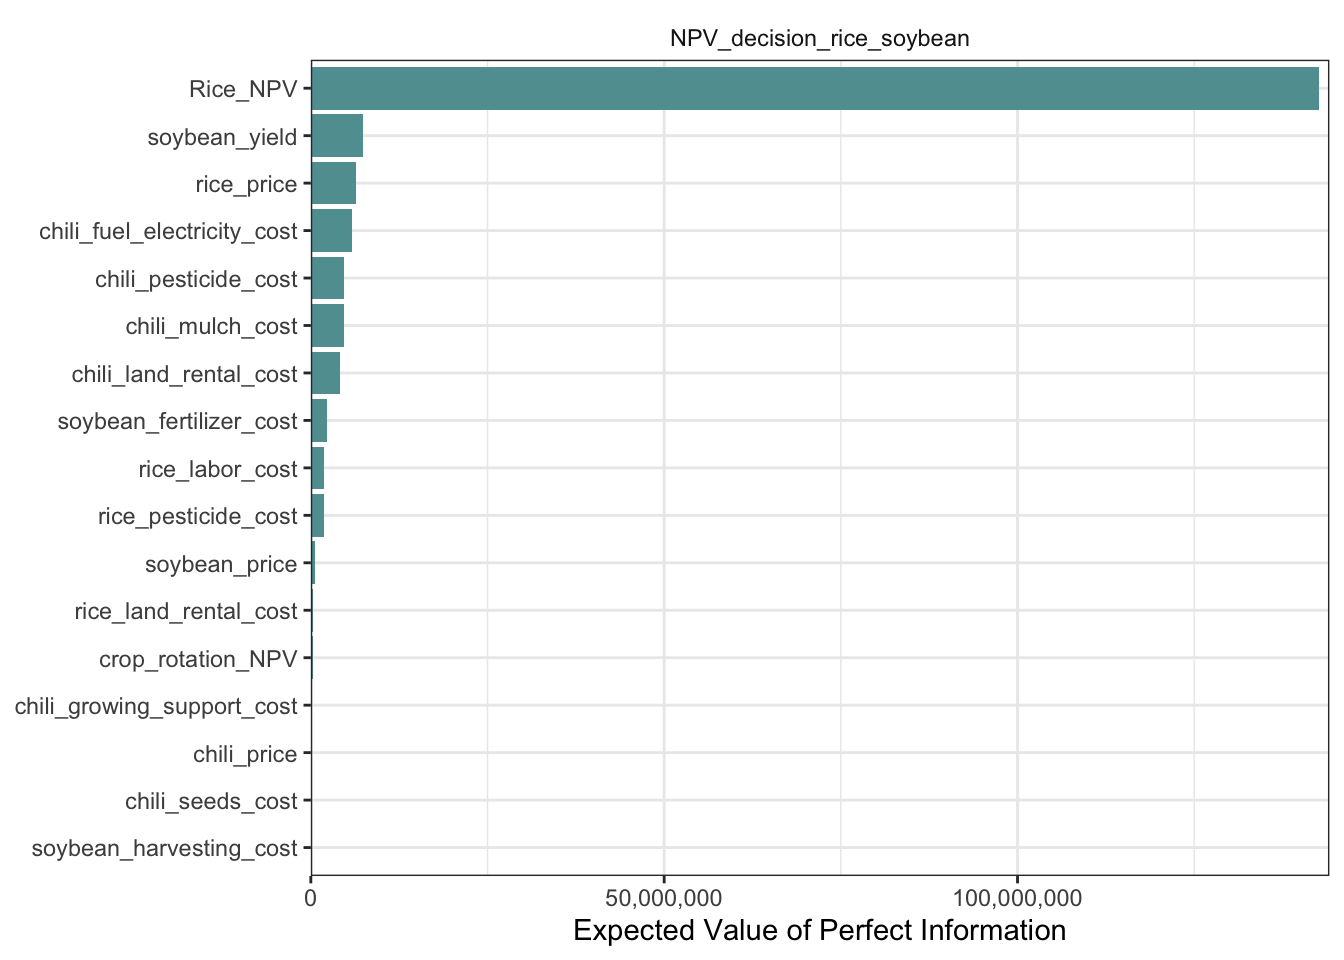
\includegraphics{Rice-farm-with-crop-rotation_files/figure-latex/unnamed-chunk-15-1.pdf}

\hypertarget{evpi-rice-and-soybean}{%
\paragraph{EVPI rice and soybean}\label{evpi-rice-and-soybean}}

\begin{Shaded}
\begin{Highlighting}[]
\NormalTok{evpi\_rice\_soybean }\OtherTok{\textless{}{-}} \FunctionTok{multi\_EVPI}\NormalTok{(}\AttributeTok{mc =}\NormalTok{ mcSimulation\_table, }\AttributeTok{first\_out\_var =} \StringTok{"rice\_soybean\_NPV"}\NormalTok{)}
\end{Highlighting}
\end{Shaded}

\begin{verbatim}
## [1] "Processing 5 output variables. This can take some time."
## [1] "Output variable 1 (rice_soybean_NPV) completed."
## [1] "Output variable 2 (rice_chili_NPV) completed."
## [1] "Output variable 3 (NPV_decision_crop_rotation) completed."
## [1] "Output variable 4 (NPV_decision_rice_soybean) completed."
## [1] "Output variable 5 (NPV_decision_rice_chili) completed."
\end{verbatim}

\begin{Shaded}
\begin{Highlighting}[]
\FunctionTok{plot\_evpi}\NormalTok{(evpi\_rice\_soybean, }\AttributeTok{decision\_vars =} \StringTok{"NPV\_decision\_rice\_soybean"}\NormalTok{)}
\end{Highlighting}
\end{Shaded}

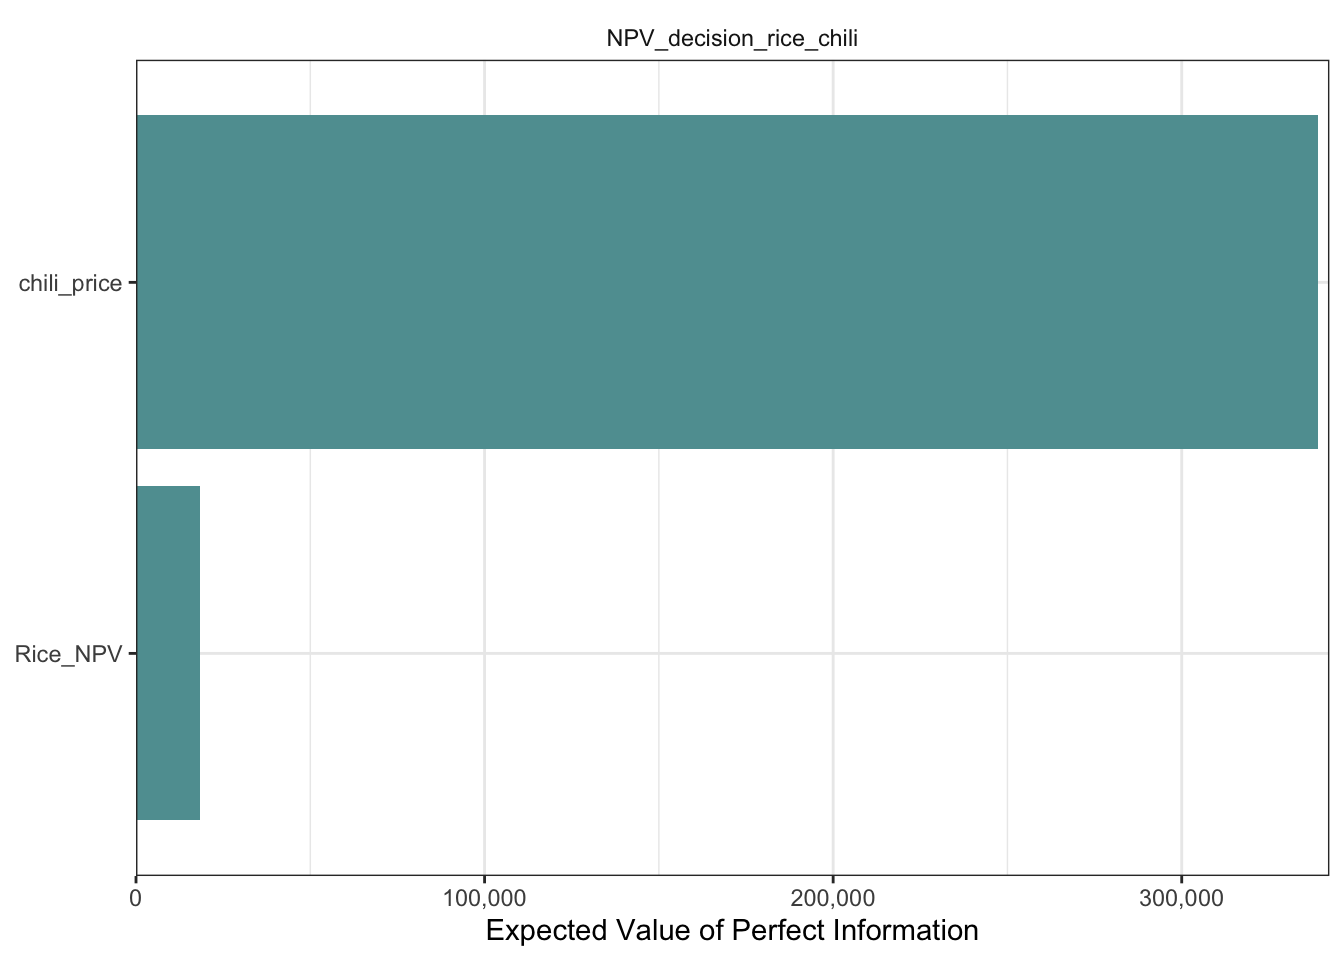
\includegraphics{Rice-farm-with-crop-rotation_files/figure-latex/unnamed-chunk-16-1.pdf}

\hypertarget{evpi-rice-and-chilli}{%
\paragraph{EVPI rice and chilli}\label{evpi-rice-and-chilli}}

\begin{Shaded}
\begin{Highlighting}[]
\NormalTok{evpi\_rice\_chili }\OtherTok{\textless{}{-}} \FunctionTok{multi\_EVPI}\NormalTok{(}\AttributeTok{mc =}\NormalTok{ mcSimulation\_table, }\AttributeTok{first\_out\_var =} \StringTok{"rice\_chili\_NPV"}\NormalTok{)}
\end{Highlighting}
\end{Shaded}

\begin{verbatim}
## [1] "Processing 4 output variables. This can take some time."
## [1] "Output variable 1 (rice_chili_NPV) completed."
## [1] "Output variable 2 (NPV_decision_crop_rotation) completed."
## [1] "Output variable 3 (NPV_decision_rice_soybean) completed."
## [1] "Output variable 4 (NPV_decision_rice_chili) completed."
\end{verbatim}

\begin{Shaded}
\begin{Highlighting}[]
\FunctionTok{plot\_evpi}\NormalTok{(evpi\_rice\_chili, }\AttributeTok{decision\_vars =} \StringTok{"NPV\_decision\_rice\_chili"}\NormalTok{)}
\end{Highlighting}
\end{Shaded}

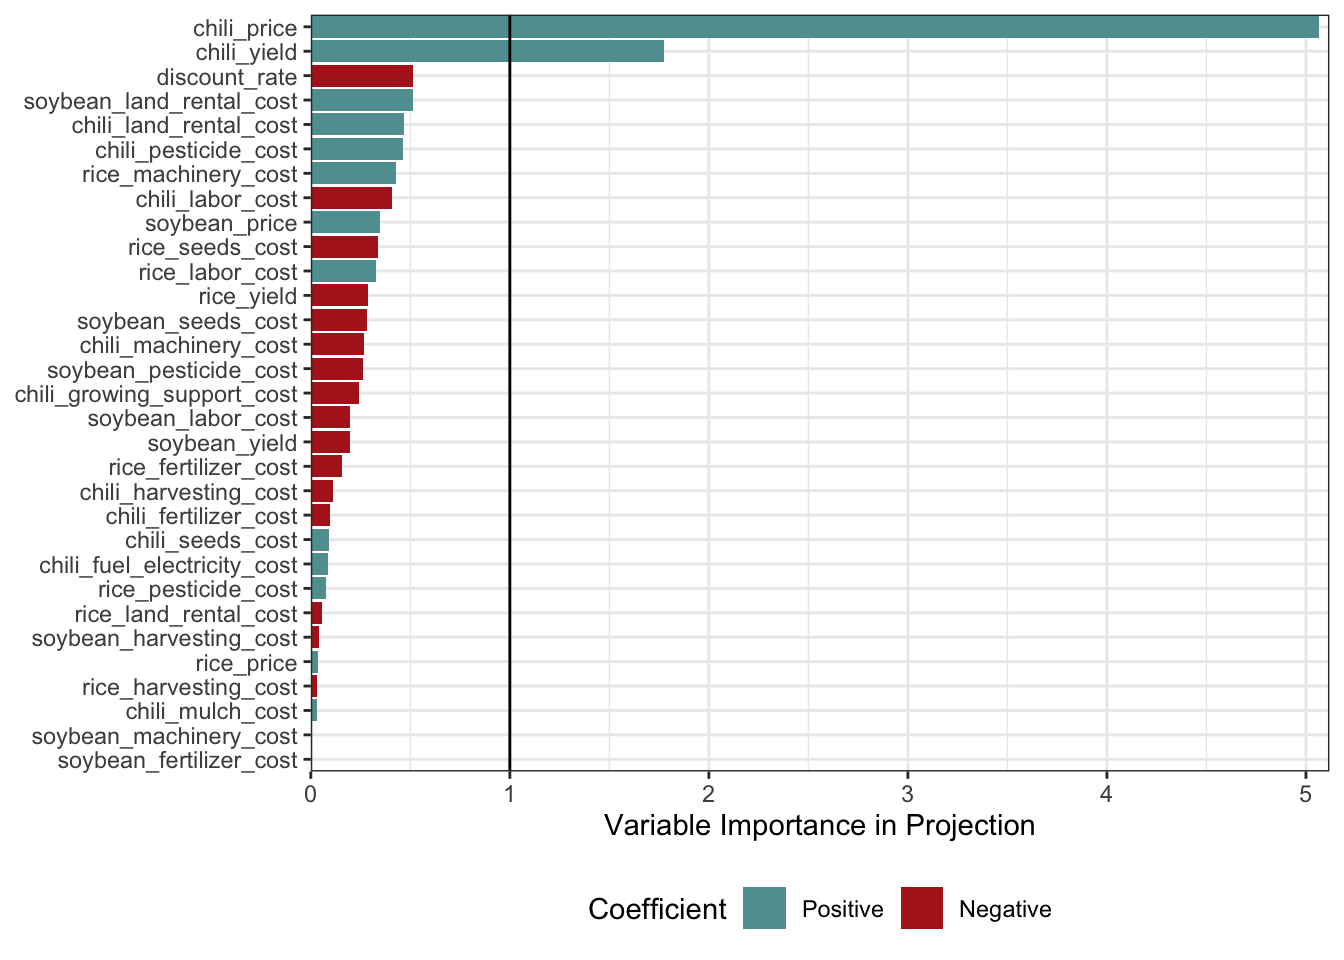
\includegraphics{Rice-farm-with-crop-rotation_files/figure-latex/unnamed-chunk-17-1.pdf}

\hypertarget{projection-to-latent-structures-pls-analysis}{%
\subsubsection{Projection to Latent Structures (PLS)
analysis}\label{projection-to-latent-structures-pls-analysis}}

\hypertarget{with-crop-rotation-of-3-crops-rice-soybean-chili-1}{%
\paragraph{With crop rotation of 3 crops
(rice-soybean-chili)}\label{with-crop-rotation-of-3-crops-rice-soybean-chili-1}}

\begin{Shaded}
\begin{Highlighting}[]
\NormalTok{pls\_result\_crop\_rotation }\OtherTok{\textless{}{-}} \FunctionTok{plsr.mcSimulation}\NormalTok{(}\AttributeTok{object =}\NormalTok{ crop\_rotation\_mc\_simulation,}
                                              \AttributeTok{resultName =} \FunctionTok{names}\NormalTok{(crop\_rotation\_mc\_simulation}\SpecialCharTok{$}\NormalTok{y)[}\DecValTok{5}\NormalTok{], }\AttributeTok{ncomp =} \DecValTok{1}\NormalTok{)}
\FunctionTok{plot\_pls}\NormalTok{(pls\_result\_crop\_rotation, }\AttributeTok{threshold =} \DecValTok{0}\NormalTok{)}
\end{Highlighting}
\end{Shaded}

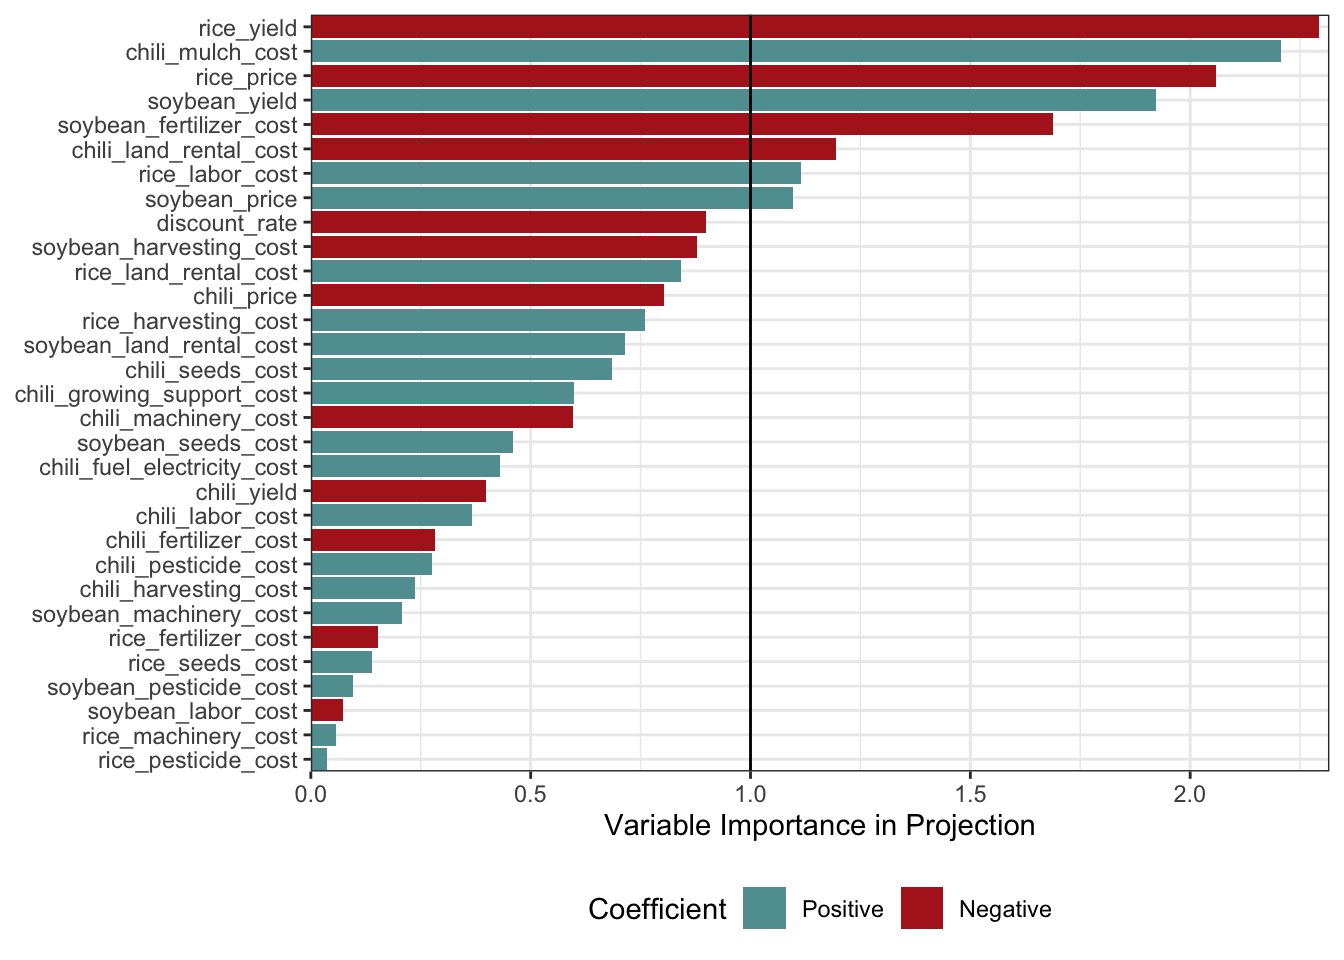
\includegraphics{Rice-farm-with-crop-rotation_files/figure-latex/unnamed-chunk-18-1.pdf}

\hypertarget{with-crop-rotation-of-rice-and-soybean-rice-soybean-rice-1}{%
\paragraph{With crop rotation of rice and soybean
(rice-soybean-rice)}\label{with-crop-rotation-of-rice-and-soybean-rice-soybean-rice-1}}

\begin{Shaded}
\begin{Highlighting}[]
\NormalTok{pls\_result\_rice\_soybean }\OtherTok{\textless{}{-}} \FunctionTok{plsr.mcSimulation}\NormalTok{(}\AttributeTok{object =}\NormalTok{ crop\_rotation\_mc\_simulation,}
                                             \AttributeTok{resultName =} \FunctionTok{names}\NormalTok{(crop\_rotation\_mc\_simulation}\SpecialCharTok{$}\NormalTok{y)[}\DecValTok{6}\NormalTok{], }\AttributeTok{ncomp =} \DecValTok{1}\NormalTok{)}
\FunctionTok{plot\_pls}\NormalTok{(pls\_result\_rice\_soybean, }\AttributeTok{threshold =} \DecValTok{0}\NormalTok{)}
\end{Highlighting}
\end{Shaded}

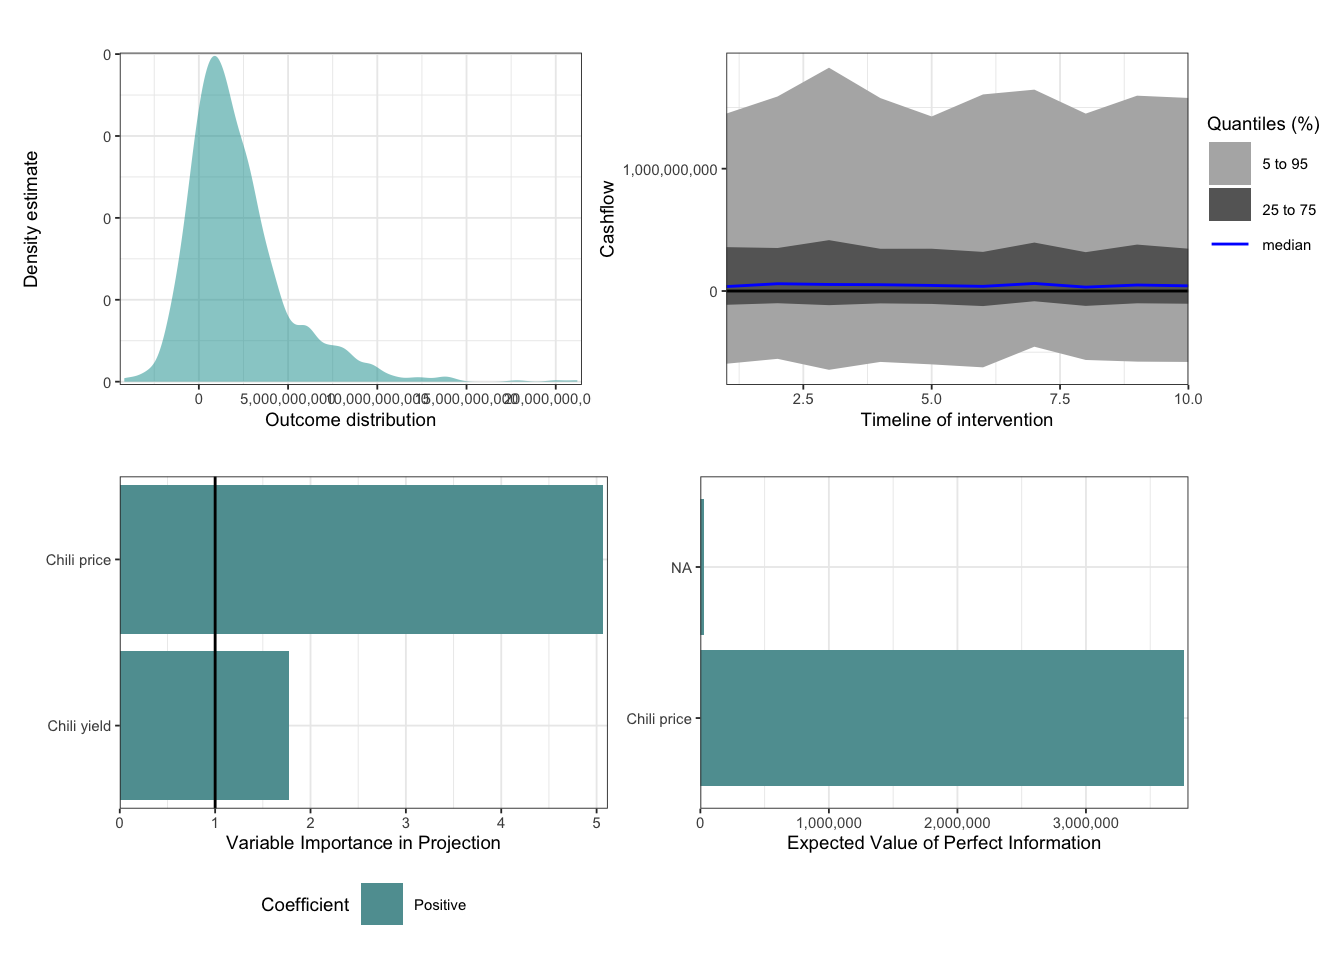
\includegraphics{Rice-farm-with-crop-rotation_files/figure-latex/unnamed-chunk-19-1.pdf}

\hypertarget{with-crop-rotation-of-rice-and-chili-rice-chili-1}{%
\paragraph{With crop rotation of rice and chili
(rice-chili)}\label{with-crop-rotation-of-rice-and-chili-rice-chili-1}}

\begin{Shaded}
\begin{Highlighting}[]
\NormalTok{pls\_result\_rice\_chili }\OtherTok{\textless{}{-}} \FunctionTok{plsr.mcSimulation}\NormalTok{(}\AttributeTok{object =}\NormalTok{ crop\_rotation\_mc\_simulation,}
                                           \AttributeTok{resultName =} \FunctionTok{names}\NormalTok{(crop\_rotation\_mc\_simulation}\SpecialCharTok{$}\NormalTok{y)[}\DecValTok{7}\NormalTok{], }\AttributeTok{ncomp =} \DecValTok{1}\NormalTok{)}
\FunctionTok{plot\_pls}\NormalTok{(pls\_result\_rice\_chili, }\AttributeTok{threshold =} \DecValTok{0}\NormalTok{)}
\end{Highlighting}
\end{Shaded}

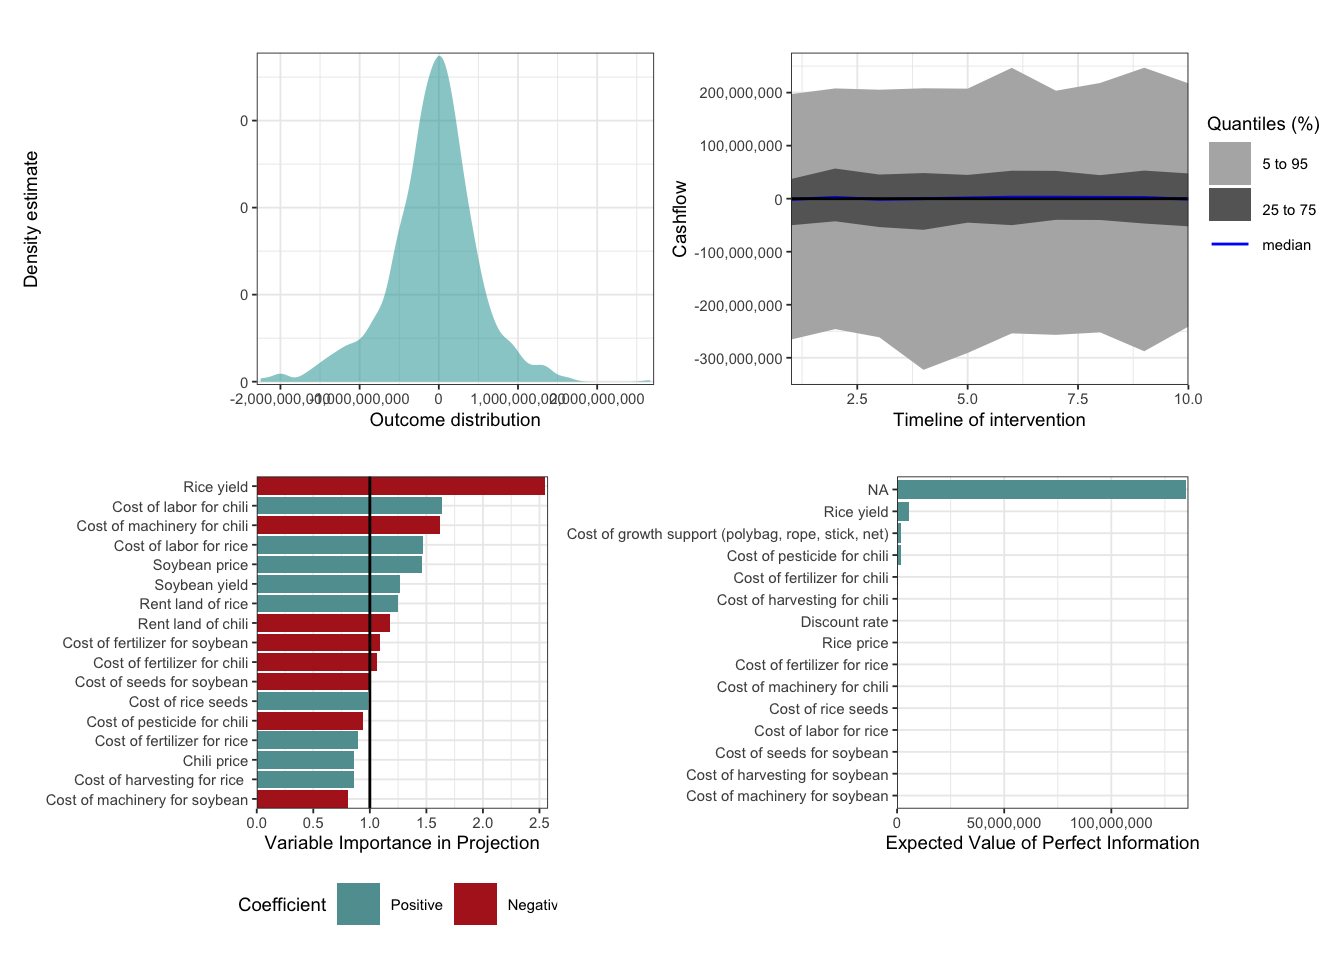
\includegraphics{Rice-farm-with-crop-rotation_files/figure-latex/unnamed-chunk-20-1.pdf}

\hypertarget{results}{%
\subsection{Results}\label{results}}

\hypertarget{with-crop-rotation-of-3-crops-rice-soybean-chili-2}{%
\subsubsection{With crop rotation of 3 crops
(rice-soybean-chili)}\label{with-crop-rotation-of-3-crops-rice-soybean-chili-2}}

\begin{Shaded}
\begin{Highlighting}[]
\FunctionTok{compound\_figure}\NormalTok{(}\AttributeTok{mcSimulation\_object =}\NormalTok{ crop\_rotation\_mc\_simulation, }
                \AttributeTok{input\_table =}\NormalTok{ input\_estimates, }\AttributeTok{plsrResults =}\NormalTok{ pls\_result\_crop\_rotation, }
                \AttributeTok{EVPIresults =}\NormalTok{ evpi\_crop\_rotation, }\AttributeTok{decision\_var\_name =} \StringTok{"NPV\_decision\_crop\_rotation"}\NormalTok{, }
                \AttributeTok{cashflow\_var\_name =} \StringTok{"cashflow\_crop\_rotation"}\NormalTok{, }
                \AttributeTok{base\_size =} \DecValTok{7}\NormalTok{)}
\end{Highlighting}
\end{Shaded}

\includegraphics{Rice-farm-with-crop-rotation_files/figure-latex/unnamed-chunk-21-1.pdf}

\hypertarget{with-crop-rotation-of-rice-and-soybean-rice-soybean-rice-2}{%
\subsubsection{With crop rotation of rice and soybean
(rice-soybean-rice)}\label{with-crop-rotation-of-rice-and-soybean-rice-soybean-rice-2}}

\begin{Shaded}
\begin{Highlighting}[]
\FunctionTok{compound\_figure}\NormalTok{(}\AttributeTok{mcSimulation\_object =}\NormalTok{ crop\_rotation\_mc\_simulation, }
                \AttributeTok{input\_table =}\NormalTok{ input\_estimates, }\AttributeTok{plsrResults =}\NormalTok{ pls\_result\_rice\_soybean, }
                \AttributeTok{EVPIresults =}\NormalTok{ evpi\_rice\_soybean, }\AttributeTok{decision\_var\_name =} \StringTok{"NPV\_decision\_rice\_soybean"}\NormalTok{, }
                \AttributeTok{cashflow\_var\_name =} \StringTok{"cashflow\_rice\_soybean"}\NormalTok{, }
                \AttributeTok{base\_size =} \DecValTok{7}\NormalTok{)}
\end{Highlighting}
\end{Shaded}

\includegraphics{Rice-farm-with-crop-rotation_files/figure-latex/unnamed-chunk-22-1.pdf}

\hypertarget{with-crop-rotation-of-rice-and-chili-rice-chili-2}{%
\subsubsection{With crop rotation of rice and chili
(rice-chili)}\label{with-crop-rotation-of-rice-and-chili-rice-chili-2}}

\begin{Shaded}
\begin{Highlighting}[]
\FunctionTok{compound\_figure}\NormalTok{(}\AttributeTok{mcSimulation\_object =}\NormalTok{ crop\_rotation\_mc\_simulation, }
                \AttributeTok{input\_table =}\NormalTok{ input\_estimates, }\AttributeTok{plsrResults =}\NormalTok{ pls\_result\_rice\_chili, }
                \AttributeTok{EVPIresults =}\NormalTok{ evpi\_rice\_chili, }\AttributeTok{decision\_var\_name =} \StringTok{"NPV\_decision\_rice\_chili"}\NormalTok{, }
                \AttributeTok{cashflow\_var\_name =} \StringTok{"cashflow\_rice\_chili"}\NormalTok{, }
                \AttributeTok{base\_size =} \DecValTok{7}\NormalTok{)}
\end{Highlighting}
\end{Shaded}

\includegraphics{Rice-farm-with-crop-rotation_files/figure-latex/unnamed-chunk-23-1.pdf}

\hypertarget{conclusion}{%
\subsection{Conclusion}\label{conclusion}}

\begin{enumerate}
\def\labelenumi{\arabic{enumi}.}
\tightlist
\item
  This project has proven that selecting the appropriate crop rotation
  between rice, soybean, and chili seem profitable for achieving optimal
  results with respect to higher income for rice farming.
\item
  The decision to rotate crops between rice and chili is still
  applicable with slightly smaller profits.
\item
  Crop rotation between rice, soybean, and rice is less efficient than
  other options with respect to sustainable income.
\end{enumerate}

\hypertarget{recommendtion}{%
\subsection{Recommendtion}\label{recommendtion}}

1.We \textbf{recommend} Indonesian smallholder farmers to implement crop
rotation either for three crops \textbf{(rice, soybean, and chili)} or
two crops \textbf{(rice and chili)} as it seems more profitable than
growing rice only all year around.

2.However, we would \textbf{not recommend} to implement crop rotation
between \textbf{rice and soybean} as it seems not so profitable.

\hypertarget{what-we-have-learned-from-this-project}{%
\subsection{What we have learned from this
project?}\label{what-we-have-learned-from-this-project}}

\begin{enumerate}
\def\labelenumi{\arabic{enumi}.}
\tightlist
\item
  Rice farming with crop rotation of soybean and chili can be
  implemented by Indonesian smallholder farmers to get higher income.
\item
  However, not every crops are profitable to be rotated with rice.
\item
  There are more uncertainties in crop rotation of rice and soybean
  compared to other scenarios. Thus, further data and research still
  needed.
\end{enumerate}

\hypertarget{reference}{%
\subsection*{Reference}\label{reference}}
\addcontentsline{toc}{subsection}{Reference}

\hypertarget{refs}{}
\begin{CSLReferences}{1}{0}
\leavevmode\vadjust pre{\hypertarget{ref-Amirrullah2019}{}}%
Amirrullah, Johanes. 2019. {``The Effect of Various Crop Rotation on the
Improvement of Soil Properties of Irrigation Paddy Field.''}

\leavevmode\vadjust pre{\hypertarget{ref-Antriyandarti2015}{}}%
Antriyandarti, Ernoiz. 2015. {``Competitiveness and Cost Efficiency of
Rice Farming in Indonesia.''} \emph{Journal of Rural Problems} 51:
74--85. \url{https://doi.org/10.7310/arfe.51.74}.

\leavevmode\vadjust pre{\hypertarget{ref-BPS2018}{}}%
BPS. 2018. {``{[}SOUH2018{]} Struktur Ongkos Usaha Tanaman Cabai Besar
Per Hektar Per Musim Tanam Di Indonesia.''}

\leavevmode\vadjust pre{\hypertarget{ref-BPS2022}{}}%
---------. 2022. {``Statistik Indonesia 2022.''}

\leavevmode\vadjust pre{\hypertarget{ref-BRIN2022}{}}%
BRIN. 2022. {``Competitiveness of Indonesian Rice Prices in the
International Market.''} In \emph{E3S Web of Conferences}. Vol. 361. EDP
Sciences. \url{https://doi.org/10.1051/e3sconf/202236101016}.

\leavevmode\vadjust pre{\hypertarget{ref-Crystal2004}{}}%
Crystal, Eric, and Peter Whittlesey. 2004. {``THE ROLE OF RICE IN
SOUTHEAST ASIA.''}

\leavevmode\vadjust pre{\hypertarget{ref-Do2020}{}}%
Do, Hoa, Eike Luedeling, and Cory Whitney. 2020. {``Decision Analysis of
Agroforestry Options Reveals Adoption Risks for Resource-Poor
Farmers.''} \emph{Agronomy for Sustainable Development} 40 (June).
\url{https://doi.org/10.1007/s13593-020-00624-5}.

\leavevmode\vadjust pre{\hypertarget{ref-Fao2018}{}}%
Fao. 2018. {``SMALL FAMILY FARMS COUNTRY FACTSHEET.''}
\href{https://www.fao.org/family-farming/data-sources/dataportrait/farm-size/en}{www.fao.org/family-farming/data-sources/dataportrait/farm-size/en}.

\leavevmode\vadjust pre{\hypertarget{ref-Harsono2020}{}}%
Harsono, Arief, Didik Harnowo, Erliana Ginting, and Dian Adi Anggraeni
Elisabeth. 2020. {``Opportunities to Achieve Self-Sufficiency.''}
\href{https://www.intechopen.com}{www.intechopen.com}.

\leavevmode\vadjust pre{\hypertarget{ref-Jagung2017}{}}%
Jagung, Kedelai. 2017. {``Nilai Produksi Dan Biaya Produksi Per Musim
Tanam Per Hektar Budidaya Tanaman Padi Sawah, Padi Ladang, Jagung, Dan
Kedelai, 2017 Uraian Padi Sawah Padi Ladang.''}

\leavevmode\vadjust pre{\hypertarget{ref-Krisdiana2021}{}}%
Krisdiana, Ruly, Nila Prasetiaswati, Imam Sutrisno, Fachrur Rozi, Arief
Harsono, and Made Jana Mejaya. 2021. {``Financial Feasibility and
Competitiveness Levels of Soybean Varieties in Rice-Based Cropping
System of Indonesia.''} \emph{Sustainability (Switzerland)} 13 (August).
\url{https://doi.org/10.3390/su13158334}.

\leavevmode\vadjust pre{\hypertarget{ref-MOALF2016}{}}%
MOALF. 2016. {``Chilli Production.''}
\url{https://www.southdevonchillifarm.co.uk/onli}.

\leavevmode\vadjust pre{\hypertarget{ref-Mucharam2020}{}}%
Mucharam, Iim, Ernan Rustiadi, Akhmad Fauzi, and Harianto. 2020.
{``Assessment of Rice Farming Sustainability: Evidence from Indonesia
Provincial Data.''} \emph{International Journal of Sustainable
Development and Planning} 15 (December): 1323--13332.
\url{https://doi.org/10.18280/ijsdp.150819}.

\leavevmode\vadjust pre{\hypertarget{ref-Schilling1999}{}}%
Schilling, Robert. 1999. {``THE SOYBEAN COMMODITY SYSTEM IN INDONESIA :
OVERVIEW AND PROPOSALS.''}

\leavevmode\vadjust pre{\hypertarget{ref-Setiartiti2021}{}}%
Setiartiti, Lilies. 2021. {``Critical Point of View: The Challenges of
Agricultural Sector on Governance and Food Security in Indonesia.''} In
\emph{E3S Web of Conferences}. Vol. 232. EDP Sciences.
\url{https://doi.org/10.1051/e3sconf/202123201034}.

\leavevmode\vadjust pre{\hypertarget{ref-Stantec2005}{}}%
Stantec. 2005. {``Helping Our Clients Prioritise Programmes and
Projects.''}

\leavevmode\vadjust pre{\hypertarget{ref-Sundari2021}{}}%
Sundari, M. T., Darsono, J. Sutrisno, and E. Antriyandarti. 2021.
{``Analysis of Chili Farming in Indonesia.''} In \emph{IOP Conference
Series: Earth and Environmental Science}. Vol. 905. IOP Publishing Ltd.
\url{https://doi.org/10.1088/1755-1315/905/1/012046}.

\leavevmode\vadjust pre{\hypertarget{ref-USDA2012}{}}%
USDA. 2012. {``INDONESIA: Stagnating Rice Production Ensures Continued
Need for Imports.''}

\leavevmode\vadjust pre{\hypertarget{ref-Wandschneider2019}{}}%
Wandschneider, Tiago, Paul Gniffke, Teddy Kristedi, Kuntoro Boga, Witono
Adiyoga, and Howard Hall N/A N/A. 2019. {``Final Report: Eastern
Indonesia Agribusiness Development Opportunities-Chilli Value Chain
Project Number.''}

\leavevmode\vadjust pre{\hypertarget{ref-Wright2005}{}}%
Wright, Jerry, Bill Wilcke, Edward Usset, Ward Stienstra, Michael
Schmitt, Gary Sands, George Rehm, et al. 2005. {``SOYBEAN FIELD BOOK.''}

\leavevmode\vadjust pre{\hypertarget{ref-Yoshida1981}{}}%
Yoshida, Shouichi. 1981. {``Fundamentals of Rice Crop Sciences.''}

\end{CSLReferences}

\end{document}
